\documentclass[aps,prb,reprint,superscriptaddress,showpacs]{revtex4-1}
\usepackage{graphicx}
\usepackage{epstopdf}
\usepackage{chemfig}

\begin{document}
\title{Theoretical Models of Hydrogen Induced Defects in Amorphous Silicon Dioxide}
    
\author{Al-Moatasem El-Sayed}
\email{al-moatasem.el-sayed.10@ucl.ac.uk}
\affiliation{Department of Physics and Astronomy and London Centre for Nanotechnology, University College London, Gower Street, London, WC1E 6BT, United Kingdom}
\author{Yannick Wimmer}
\email{wimmer@iue.tuwien.ac.at}
\affiliation{Institute for Microelectronics, Technische Universit\"{a}t Wien, A-1040
Vienna, Austria}
\author{Wolfgang Goes}
\email{goes@iue.tuwien.ac.at}
\affiliation{Institute for Microelectronics, Technische Universit\"{a}t Wien, A-1040
Vienna, Austria}
\author{Tibor Grasser}
\email{grasser@iue.tuwien.ac.at}
\affiliation{Institute for Microelectronics, Technische Universit\"{a}t Wien, A-1040
Vienna, Austria}
\author{Valery V. Afanas'ev}
\email{valeri.afanasiev@fys.kuleuven.be}
\affiliation{Department of Physics, University of Leuven, Celestijnenlaan 200D, 3001 Leuven, Belgium}
\author{Alexander L. Shluger}
\email{a.shluger@ucl.ac.uk}
\affiliation{Department of Physics and Astronomy and London Centre for Nanotechnology, University College London, Gower Street, London, WC1E 6BT, United Kingdom}
\author{John Smith}
\email{a.shluger@ucl.ac.uk}
\affiliation{Department of Physics and Astronomy and London Centre for Nanotechnology, University College London, Gower Street, London, WC1E 6BT, United Kingdom}

\date{\today}
\begin{abstract}
We used Density Functional Theory (DFT) calculations to model the interaction of hydrogen atoms and molecules with strained bonds and neutral oxygen vacancies in amorphous silica (a-SiO$_2$). The results demonstrate that the interaction of atomic hydrogen with strained \mbox{Si--O} bonds in defect-free a-SiO$_2$ networks results in the formation of two distinct defect structures referred to as the [SiO$_4$/H]$^0$ and the hydroxyl E$^\prime$ center. To study the distribution of each defect's properties, up to 116 configurations of each center were calculated. We show that the hydroxyl E$^\prime$ center can be thermodynamically stable in the neutral charge state. In order to understand the origins and reactions of this defect, different mechanisms of formation, passivation and de-passivation have been investigated. The interaction of H with a single oxygen vacancy in a-SiO$_2$ was studied in 144 configurations, all resulting in the hydrogen bridge defect. The reaction of the hydrogen bridge defect with the second H atom is barrier-less and fully passivates the O vacancy. The latter defect reacts with atomic H with a small barrier, restoring the hydrogen bridge defect. These results provide a better understanding of how atomic and molecular hydrogen can both passivate existing defects and create new electrically active defects in amorphous silica matrices.

\end{abstract}

\pacs{71.55.Jv,72.15.Rn,71.23.An}
\keywords{Hydrogenic Defects, Hydroxyl E$^\prime$ Center, Hydrogen Bridge}
\maketitle

\section{Introduction}

Hydrogen is well know as a defect passivator in amorphous SiO$_2$ (a-SiO$_2$) and has been exploited in this role by both the microelectronics and optics communities to suppress electrically and optically detrimental defect states (such as the $P_\mathrm{b}$ and $E'$ centers).~\cite{LENAHAN08} In addition, it is also known to take part in various chemical and physical processes at Si/SiO$_2$ interfaces and in bulk amorphous SiO$_2$.~\cite{pobegen_h,cartier_depassivation,stathis_depassivation,hydrogen_ria,hydrogen_breakdown} Examples of hydrogen and water induced effects include hydrolytic weakening of quartz and minerals,~\cite{hobbs_h} degradation phenomena in optical fibers~\cite{griscom_fibers} and in SiO$_2$-insulated electronic devices, such as radiation damage,~\cite{revesz,mclean_radiation,griscom_radiation1} as well as injection-induced~\cite{dimaria_injection} and bias-temperature instabilities.~\cite{helms_bti,pobegen_h_nbti} Hydrogen-complexed defects have been identified using electron spin resonance (ESR) methods, such as the hydrogen bridge,~\cite{eprime_4_1,eprime_4_2} the 74 G-, and the 10.4 G-doublet center.~\cite{CONLEY92,LENAHAN08,kannan_hydrogen_epr} Due to the technological importance of a-SiO$_2$, these defects are the subject of intense research efforts across a range of disciplines, but despite these efforts, the role of atomic hydrogen in silica degradation processes is still poorly understood.

During radiation-induced processes, radiolytic hydrogen atoms can be released into the glassy a-SiO$_2$ core of optical fibers. These H atoms have been postulated to interact with the a-SiO$_2$ matrix, generating \mbox{O--H} groups which are responsible for increased radiation induced attenuation (RIA) at $\approx$ 1380 nm.~\cite{girard_sio2_review} In contrast, hydrogen (and deuterium) loading of optical fibers has been shown to reduce RIA at visible to near ultra-violet (UV) wavelengths, although these fibers show the same aforementioned increased RIA at higher wavelengths.~\cite{hydrogen_ria} The reduction in RIA after hydrogen loading is thought to be due to hydrogen passivation of the defects responsible for RIA at visible wavelengths. Radiolysis~\cite{shkrob1,shkrob2} and photolysis of silica glass -- e.g. using ArF and F$_2$ lasers~\cite{skuja_hydrogen,skuja_hydrogen2,skuja_hdiffusion} -- readily creates high concentrations of atomic hydrogen which diffuses rapidly through the silica network with activation energies of about 0.2 eV.~\cite{kajihara_hydrogen,skuja_hdiffusion} These mobile atoms interact with point defects in a-SiO$_2$, such as Si dangling bonds and passivated \mbox{Si--H} bonds, forming several H-related paramagnetic centers characterized by ESR.~\cite{vitko_hydrogen,radzig_surface,skuja_hydrogen,skuja_hydrogen2} In particular, a 0.08 mT doublet due to proton hyperfine splitting has recently been assigned to a Si dangling bond coordinated by two bridging oxygens and an OH group (called E$^\prime$(OH)-center), which is thought to result from a reaction of H$^0$ with electronically excited strained \mbox{Si--O} bonds.~\cite{skuja_hydrogen} Although H-related defects are abundant in optical-grade silica, their formation mechanisms remain largely unknown. 

Defect passivation by hydrogen has also long been exploited in the fabrication of electronic devices, with anneals in H$_2$ and forming gas routinely employed to suppress electrically detrimental states. However, analysis of defects in the most chemically pure a-SiO$_2$ layers grown by thermal oxidation of silicon and, therefore, not compromised by the presence of other impurities, has also shown that a supply of hydrogen during thermal treatment or illumination may lead to formation of additional densities of intrinsic network defects.~\cite{pobegen_h_nbti} Critically, they exceed the density of the same defects in identical a-SiO$_2$ films processed in the absence of hydrogen.~\cite{wilde_hdefects2} These additional defects are also predominantly Si dangling bonds in SiO$_2$ (E$^\prime$-type centers: \setatomsep{2em}\chemfig{O_3~\lewis{0.,Si}}\hspace{2 pt} entity, where the dot symbolizes an unpaired electron~\cite{asio2_hetrap3}) or at the Si/SiO$_2$ interface (P$_b$-type centers: \chemfig{Si_3~\lewis{0.,Si}}\hspace{2 pt} entity~\cite{stesmans_etrap,afanasev_pb}), suggesting that H-induced bond rupture occurs in the ostensibly defect-free a-SiO$_2$ network and at the Si/a-SiO$_2$ interface. Accumulation of hydrogen inside the a-SiO$_2$ films revealed by a variety of methods firmly supports this conjecture and further suggests that the broken bonds are passivated by hydrogen.~\cite{rivera_hdefect,wilde_hdefect} Although the \mbox{Si--O} bond rupture was initially correlated with the presence of protonic species~\cite{afanasev_prb,afanasev_protonic1} formed by hole trapping~\cite{AFANASEV01B} or hydrogen ionization at the Si/SiO$_2$ interface,~\cite{etrapping_1} the involvement of H$^0$ should also be considered since it is far more abundant than radiolytic protons. 

%In electronic devices, hydrogen is known for its ability to passivate defects and impurities. Anneals in H$_2$ and forming gas are routinely employed in electronic device fabrication processes to suppress electrically detrimental states. Despite its well-known healing role, hydrogen has been implicated in a number of electronic device reliability issues, such as stress induced leakage current ~\cite{BLOECHL99} and bias temperature instabilities.~\cite{pobegen_h,helms_bti} Hydrogen in the form of protons have been implicated in the generation of defect precursors in Si/a-SiO$_2$ systems.~\cite{afanasev_prb,afanasev_protonic1}

Previous theoretical studies have shown that neutral hydrogen, both atomic and molecular, interacts negligibly with defect-free SiO$_2$.~\cite{blochl_vacancies,yokozawa_h} Moreover, neutral interstitial hydrogen atoms have been shown to be thermodynamically unstable across the entire band gap in both crystalline~\cite{blochl_vacancies} and amorphous~\cite{godet_hydrogen} SiO$_2$ and exhibit a negative-U behavior.~\cite{godet_hydrogen,robertson_oxides} Nevertheless, atomic hydrogen, both radiolytic ~\cite{griscom_hydrogen} or injected from metal electrodes in the process of anneal, is often detected in quartz and in a-SiO$_2$ due to inefficient electron transfer to/from electrodes or impurities defining the Fermi level.~\cite{griscom_hydrogen} In contrast to defect-free a-SiO$_2$, theoretical studies have shown that both atomic and molecular hydrogen interact with point defects in SiO$_2$. Using a cluster model and post Hartree-Fock (HF) methods, Edwards \emph{et al.} studied the interaction of hydrogen molecules with E$^\prime$-type defects (i.e., an \setatomsep{2em}\chemfig{O_3~\lewis{0.,Si}}\hspace{2 pt} moiety) in $\alpha$-quartz.~\cite{edwards_h2} The clusters studied were terminated with O--H groups, with the terminating H atoms fixed in space. They showed that the H$_2$ molecule dissociates at an E$^\prime$ center to leave behind a free H atom and an Si--H bond, passivating the 3-coordinated Si with a barrier of 0.78 eV. This calculated barrier is higher than the barrier extracted experimentally by Li \emph {et al.},~\cite{h2crack_li} although both experiment and theory find this passivation reaction to be endothermic. Using similar cluster models and various post HF methods, Kurtz \emph{et al.} then showed that the barrier for H$_2$ dissociation at E$^\prime$ centers is closer to 0.3--0.4 eV, when nuclear tunneling of H is taken into consideration.~\cite{kurtz_h2} Their results also showed that the various post HF methods gave different stabilities for the reactants and products, with all the higher levels of theory predicting the H$_2$ dissociation reaction at E$^\prime$ centers to be endothermic as was the case with Edwards' studies. Hybrid density functional theory calculations on small clusters by Lopez \emph{et al.} also indicate the H$_2$ cracking reaction at E$^\prime$ centers to be endothermic with a barrier of less than 0.5 eV.~\cite{h2crack_sidb_ts} In a recent study we have demonstrated that H atoms can break strained \mbox{Si--O} bonds in continuous a-SiO$_2$ networks, resulting in a new defect consisting of a threefold-coordinated Si atom with an unpaired electron facing a hydroxyl group (a so called hydroxyl E$^\prime$ center).~\cite{aelsayed_prl} However, the thermodynamic stability of this defect has not been fully analyzed and the interaction of atomic H with O deficient a-SiO$_2$ matrix has not been considered in detail in previous publications.

In this paper, we use \emph{ab initio} modeling to further investigate the interaction of hydrogen with both continuous a-SiO$_2$ network and with oxygen vacancies. We find that reactions of atomic H with \mbox{Si--O} bonds in the bulk of stoichiometric a-SiO$_2$ can create two distinct defect configurations, which we call the [SiO$_4$/H]$^0$ (see Fig. \ref{fig:sio2_h_config}b) and the hydroxyl E$^\prime$ center (see Fig. \ref{fig:sio2_h_config}c). Hydrogen's reactions with O vacancies lead to creation of an analog to the well-known hydrogen bridge defect in $\alpha$-quartz~\cite{blochl_vacancies,alkauskas_h} where an unpaired electron faces an \mbox{Si--H} bond rather than a hydroxyl group (see Fig. \ref{fig:h_bridge}b). We then investigate the thermodynamic stability of these defects and their passivation and de-passivation reactions with atomic and molecular hydrogen species. 

\section{Details of Calculations}
\label{sec:calc_details}

We assume that atomic or molecular hydrogen injected into a-SiO$_2$ network, e.g., from metal electrodes or created inside in the result of radiation-induced processes or chemical reactions, can explore the network due to its low diffusion barrier in a-SiO$_2$ networks.~\cite{kajihara_hydrogen,skuja_hdiffusion} As we have demonstrated in Ref. \cite{aelsayed_prl}, elongated \mbox{Si--O} bonds are prone to thermally activated chemical reaction with atomic H with the reaction barrier ranging between 0.5 and 1.3 eV. This barrier is higher for shorter \mbox{Si--O} bonds. However, the concentration of strained \mbox{Si--O} bonds is small and depends on the sample preparation. The wide distribution of barrier energies and small concentration of precursor sites emphasizes the importance of studying large numbers of a-SiO$_2$ samples to obtain statistically meaningful results. The same applies to O-vacancies, which exhibit a wide distribution of \mbox{Si--Si} distances, dependent on the position in the network and local environment.~\cite{asio2_3}

The calculations presented in this work make use of classical force-fields to generate a-SiO$_2$ samples followed by \emph{ab initio} calculations to characterize the H interactions with the a-SiO$_2$ network. The ReaxFF force-field~\cite{reaxff_sisio} was used to generate 116 periodic models of amorphous SiO$_{2}$, each containing 216 atoms. ReaxFF was parameterized to reproduce the properties of various silica polymorphs, small silica clusters and silicon polymorphs.~\cite{reaxff_h2o} All classical atomistic simulations were performed using the LAMMPS code.~\cite{lammps} Defect-free continuum random network a-SiO$_2$ structures were produced using molecular dynamics simulations by melting crystalline SiO$_2$ structures and quenching the melt into an amorphous state, as described in a previous publication.~\cite{aelsayed_prb} Densities of the ReaxFF a-SiO$_2$ structures ranged from 1.99 to 2.27 g cm$^{-3}$, averaging at 2.16 g cm$^{-3}$. These values fall within the range of densities known for a-SiO$_2$.  

Density functional theory (DFT), implemented in the CP2K code, was used to further optimize the ReaxFF structures and calculate their electronic structures.~\cite{cp2k_code} All 116 defect-free ReaxFF structures were optimized and then used to study the interaction of H with a-SiO$_2$ network, with results described in section \ref{sec:defect_free}. In addition, all oxygen atoms were removed from a single a-SiO$_2$ structure to create 144 neutral oxygen vacancies, whose interaction with hydrogen is described in section \ref{sec:vacancies}. The non-local functional PBE0\_TC\_LRC was used in all calculations with a cutoff radius of 2.0 {\AA} for the truncated Coulomb operator.~\cite{tc_lrc} Inclusion of Hartree-Fock exchange provides a more accurate description of the band gap and the localized states that may be involved in charge trapping processes. The CP2K code uses a Gaussian basis set with an auxiliary plane-wave basis set.~\cite{cp2k_gpw} Employing a Gaussian basis set has the advantage of allowing one to use fast analytical integration schemes, developed in quantum chemical methods, to calculate most of the Kohn-Sham matrix elements. The use of an auxiliary plane wave basis set allows one to use fast Fourier transform algorithms for rapid convergence of the long range Hartree terms. A double-$\zeta$ Gaussian basis set with polarization functions~\cite{dzv_basis} was employed in conjunction with the Goedecker-Teter-Hutter (GTH) pseudopotential.~\cite{gth_pp} Calculating hyperfine interactions necessitated the use of all electron basis sets using the Gaussian and augmented plane-wave (GAPW) approach. The basis sets with contraction schemes of (8831/831/1),(8411/411/11) and 6-311G** were used for silicon,~\cite{si_basis_crystal} oxygen~\cite{o_basis_crystal} and H,~\cite{li_basis_6311gxx} respectively. The plane wave cut-off was set to 5440 eV (400 Ry).

To reduce the computational cost of non-local functional calculations, the auxiliary density matrix method (ADMM) was employed.~\cite{admm} The density is mapped onto a much sparser Gaussian basis set containing less diffuse and fewer primitive Gaussian functions than the one employed in the rest of the calculation. This allows the Hartree-Fock exchange terms, whose computational expense scales to the fourth power of the number of basis functions, to be calculated on a much smaller basis set than the rest of the calculation and therefore much faster. 

All geometry optimizations were performed using the BFGS optimizer to minimize forces on atoms to within 37 pN (2.3 $\times 10^{-2}$ eV {\AA}$^{-1}$). Cell vectors were not allowed to relax from their ReaxFF values. Barriers between configurations were calculated using the climbing image nudged elastic band method (CI-NEB).~\cite{neb1,neb2} Linear interpolation was used to generate 10 images between an initial and final configuration to be used as the band in the CI-NEB trajectory for each calculated barrier, with each of the images connected by a spring with a force constant of 2 eV {\AA}$^2$.

To assess the thermodynamic stability of the defects studied, their formation energies were calculated as:
\begin{equation}
E_{for}(\epsilon_F)=E_{defect}-(E_{bulk}+E_{H^0})+q(\epsilon_F + \Delta V) + E_{corr},
\label{eq:formation_fermi}
\end{equation}
where $E_{defect}$ is the total energy of the defective system, $E_{bulk}$ is the energy of the defect-free system, $E_{H^0}$ is the energy of a H atom calculated using the same method, $q$ is the charge state of the defect, $\epsilon_F$ is the Fermi level referenced to the top of the a-SiO$_2$ valence band, $\Delta V$ is a potential alignment term, and $E_{corr}$ is a correction term for the periodic interaction between localized charges in the charged systems. The $\Delta V$ term was found to be negligible ($< 0.05$ eV) and was therefore ignored. The Lany and Zunger method for charge correction was chosen for its ability to describe the interaction between a localized charge and extended delocalized screening charge density, which comes out of DFT calculations of charged cells.~\cite{lany_zunger,finite_size} The analytic form of the charge correction is the same for all the defects, irrespective of the character of localization, and is calculated as:
\begin{equation}
E_{corr}=\left [ 1 - \frac{\pi}{3 \alpha}\left (1-\frac{1}{\varepsilon}\right)\right ]\frac{q^2\alpha}{2 \varepsilon L},
\label{eq:ecorr}
\end{equation}
where $\varepsilon$ is the macroscopic dielectric constant of SiO$_2$ (3.9~\cite{sio2_dielectric}), q is the charge of the cell, $\alpha$ is the Madelung constant for a single charge in a periodic array and L is the supercell length. 

\section{Results of calculations}
\subsection{Atomic Hydrogen in Pure, Stoichiometric a-SiO$_2$}

\label{sec:defect_free}
\begin{figure}[h!]
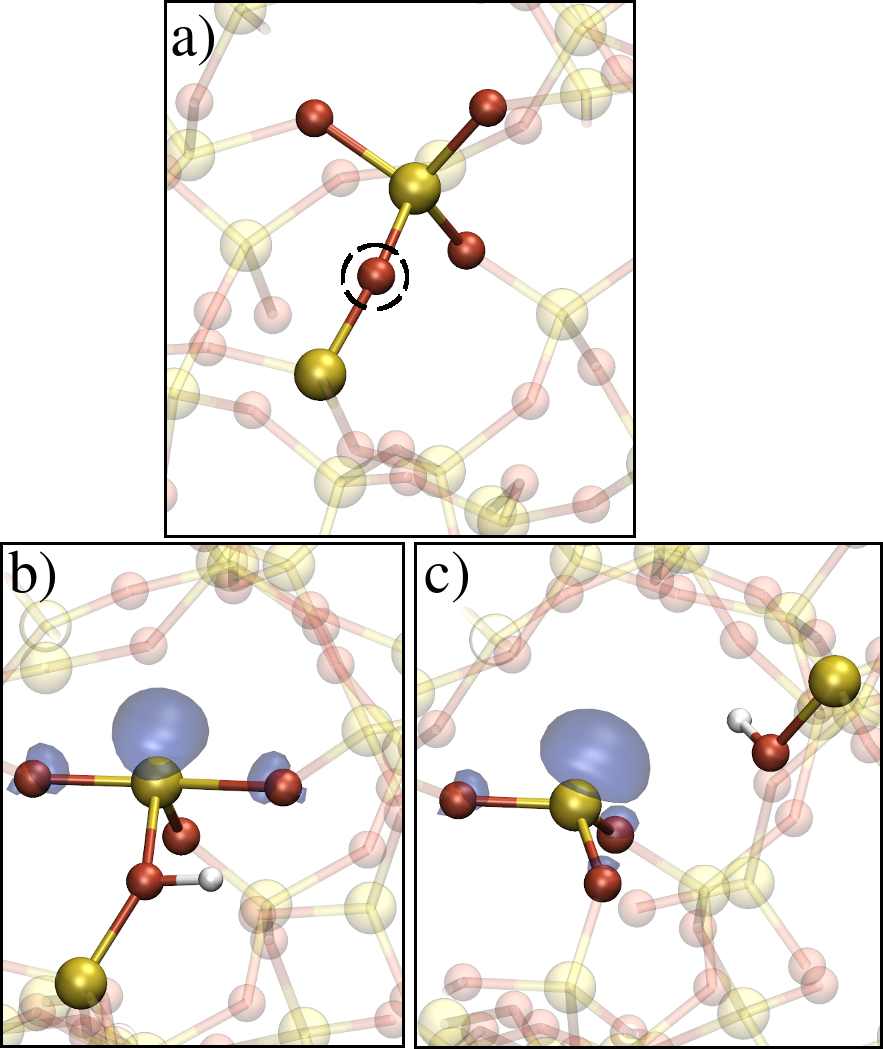
\includegraphics{hydroxyl_eprime_configurations2.png}
\caption{Atomic configuration and spin density of the two hydrogen induced defect configurations and their precursor. The Si atoms are the bigger yellow balls, the O atoms are the smaller red balls and the H atom is the small white ball in each configuration. The spin densities are the blue, transparent polyhedra. a) An unperturbed SiO$_4$ tetrahedron. The circled bridging O center has a statistically long \mbox{Si--O} bond which acts as a precursor for the following hydrogen defect configurations. b) The [SiO$_4$/H]$^0$ center. Although the \mbox{Si--O} bond between the central Si and the O to which the H is bound is still intact, it is highly strained and averages 1.99 {\AA}. The spin density is localized on the central Si atom and two of its O neighbors. A proton is attached to the bridging O at the bottom of the configuration. c) The hydroxyl E$^\prime$ center. A 3-coordinated Si where the spin density is localized on the Si and its three O neighbors. The 3-coordinated Si faces a hydroxyl group.}
\label{fig:sio2_h_config}
\end{figure}

It is well established that if H atom is further than 2.0 {\AA} away from its neighbors, it occupies an interstitial position and becomes mobile at temperatures exceeding 30 K both in quartz and in a-SiO$_2$.~\cite{skuja_hdiffusion,godet_hydrogen,blochl_vacancies} However, an a-SiO$_2$ network contains strained bonds, usually associated with local structures with \mbox{Si--O} bond lengths and \mbox{Si--O--Si} angles at the tails of corresponding distributions far from their average values. These bonds are thought to cleave more easily in some of the radiation-induced processes as well as to be more chemically active towards interaction with water and other molecules.~\cite{awazu} With this in mind, we explore the potential energy landscape of a-SiO$_2$ with respect to the interaction with H atoms more thoroughly. Since \mbox{O--H} bonds have a typical length of about 1.0 {\AA}, calculations were carried out where H atoms were initially placed 1.0 {\AA} away from short ($< 1.60$ {\AA}) and long ($> 1.65$ {\AA}) \mbox{Si--O} bonds in a perfect a-SiO$_2$ network (see Fig. \ref{fig:sio2_h_config}a). The subsequent geometry optimization resulted in discovery of two distinct defect centers described below.

\subsubsection{[SiO$_4$/H]$^0$ Center}

The first defect center resembles a proton bound to a bridging oxygen atom with an unpaired electron trapped on an adjacent four-coordinated Si atom (see Fig. \ref{fig:sio2_h_config}b) and shall be referred to as the [SiO$_4$/H]$^0$ center for the remainder of the paper. This defect was found to be efficiently generated when neutral H atoms were initially placed near short \mbox{Si--O} bonds. We note that it is similar to the [SiO$_4$/Li]$^0$ center described in Ref. \cite{aelsayed_prb}. The energy required for ionizing the H atom into the a-SiO$_2$ conduction band is compensated by the energy gain due to the structural relaxation associated with opening of the \mbox{O--Si--O} angle (see Fig. \ref{fig:sio2_h_config}b), the formation of the \mbox{O--H} bond, and the Coulomb attraction between the electron localized on Si and the hydrogen. 

To further characterize this defect, we produced 80 different configurations of the [SiO$_4$/H]$^0$. The proton is located $0.97$ {\AA} on average away from the bridging O atom. The electron trapping on Si is accompanied by the opening of an \mbox{O--Si--O} angle to an average of 165$^\circ$, ranging from 162$^\circ$ to 170$^\circ$, with the two \mbox{Si--O} bonds associated with this angle extending to an average of 1.76 {\AA}, ranging from 1.72 {\AA} to 1.88 {\AA}. The \mbox{Si--O} bond to which the H binds to extends to an average of 1.99 {\AA}, while the remaining \mbox{Si--O} bond in the SiO$_4$ tetrahedron remains at an average of 1.64 {\AA}. The character of electron trapping on the \mbox{O--Si--O} angle is notably similar to the intrinsic electron traps previously reported in the literature~\cite{electron_trap_sio2,aelsayed_prb}. A one-electron state of the unpaired electron is located in the band gap, 3.5 eV above the a-SiO$_2$ valence band on average, and is mainly Si `sp' in character with a contribution from O `p' orbitals. The hyperfine interactions of the atoms surrounding the defect with the unpaired electron have been calculated in seven configurations of this center. The splitting from the H$^1$ averages at 0.02 mT and ranges over 0.03 mT. However, the splitting from the Si$^{29}$ averages at 31 mT. 

The total energy of the system containing the [SiO$_4$/H]$^0$ center is very similar to that of the interstitial H atom, ranging from being 0.2 eV more to 0.1 eV less stable than the interstitial H atom. We have calculated the barrier to forming this defect from an interstitial H atom using CI-NEB and 10 interpolated images between an interstitial configuration and the [SiO$_4$/H]$^0$ center. The average value of this barrier from 3 different calculations is 1.3 eV. 


\subsubsection{Hydroxyl E$^\prime$ Center}

The second defect configuration, which we call the hydroxyl E$^\prime$ center, typically forms when a H atom interacts with elongated (about 1.65 {\AA}) \mbox{Si--O} bonds (see Fig. \ref{fig:sio2_h_config}c). The structure of this defect has been characterized previously.~\cite{aelsayed_prl} Briefly, it resembles an E$^\prime$ center, i.e., a 3-coordinated Si atom with an unpaired electron,~\cite{rudra_eprime} facing a hydroxyl group. The H atom breaks a strained \mbox{Si--O} bond, forming an \chemfig{O_3~\lewis{0.,Si}}\hspace{2 pt} moiety and a hydroxyl group (see Fig. \ref{fig:sio2_h_config}c). The \mbox{Si--O} bonds of the \chemfig{O_3~\lewis{0.,Si}}\hspace{2 pt} moiety average at 1.65 {\AA} while the distance between the Si and the O from which it dissociated averages at 2.63 {\AA} forming a very wide distribution which can be seen in Fig. \ref{fig:hydroxyl_geometry}c. 

\begin{figure}
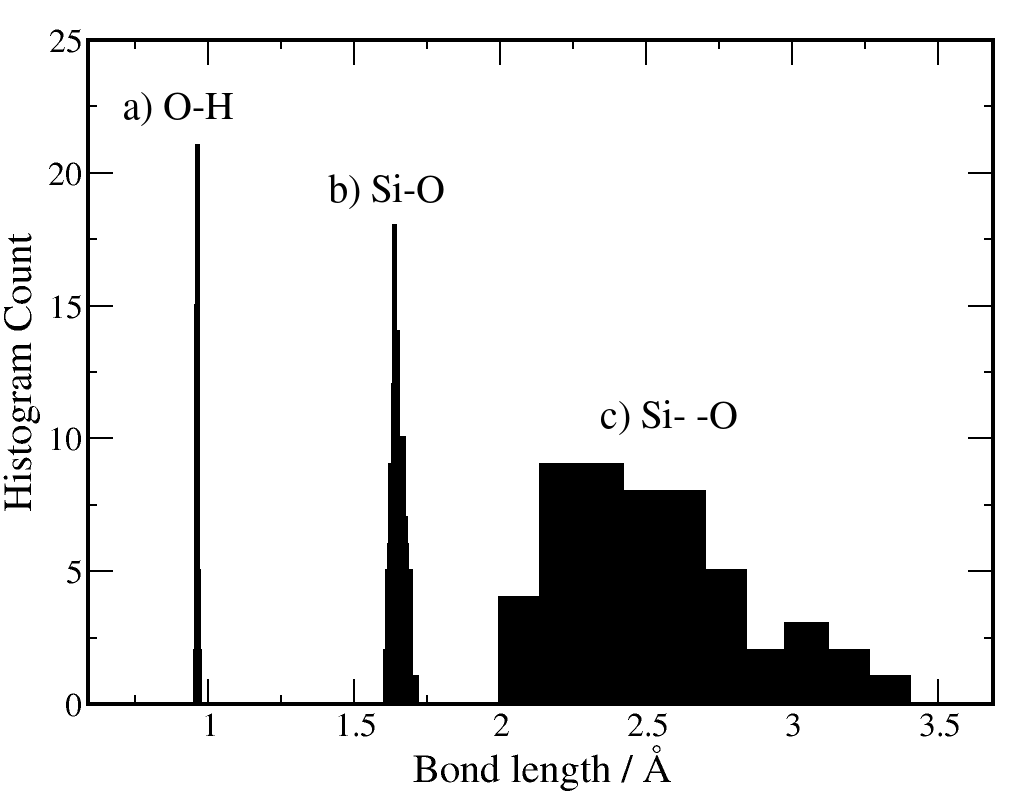
\includegraphics{hydroxyl_eprime_distribution.png}
\caption{Histograms of the bond length distributions around the hydroxyl E$^\prime$ center. a) Distribution of the \mbox{O--H} bonds of the hydroxyl group belonging to the hydroxyl E$^\prime$ center. b) Distribution of the three \mbox{Si--O} bond lengths around the 3-cooordinated Si of the hydroxyl E$^\prime$ center. c) Distribution of the \mbox{Si- -O} distance where the Si belongs to the 3-coordinated Si and the O belongs to the hydroxyl group (see Fig. \ref{fig:sio2_h_config}). Note that \mbox{- -} indicates a non-bonding interaction. }
\label{fig:hydroxyl_geometry}
\end{figure}

The average Mulliken spin moment of the 3-coordinated Si is 0.90, ranging from 0.84 to 0.98, indicating that the unpaired spin is highly localized on it. The Si dangling bond introduces a one-electron state 3.1 eV above the a-SiO$_2$ valence band on average, almost resonant with the top of the Si valence band (c.f. Si/SiO$_2$ valence band offset~\cite{sisio2_vb_offset}). Figure \ref{fig:sio2_h_dos}a shows the distribution of positions of the occupied and unoccupied one-electron levels of the hydroxyl E$^\prime$ center within the a-SiO$_2$ band gap. It is interesting to note that from the 116 configurations, a normal distribution of electronic states emerges. 

\begin{figure}[h!]
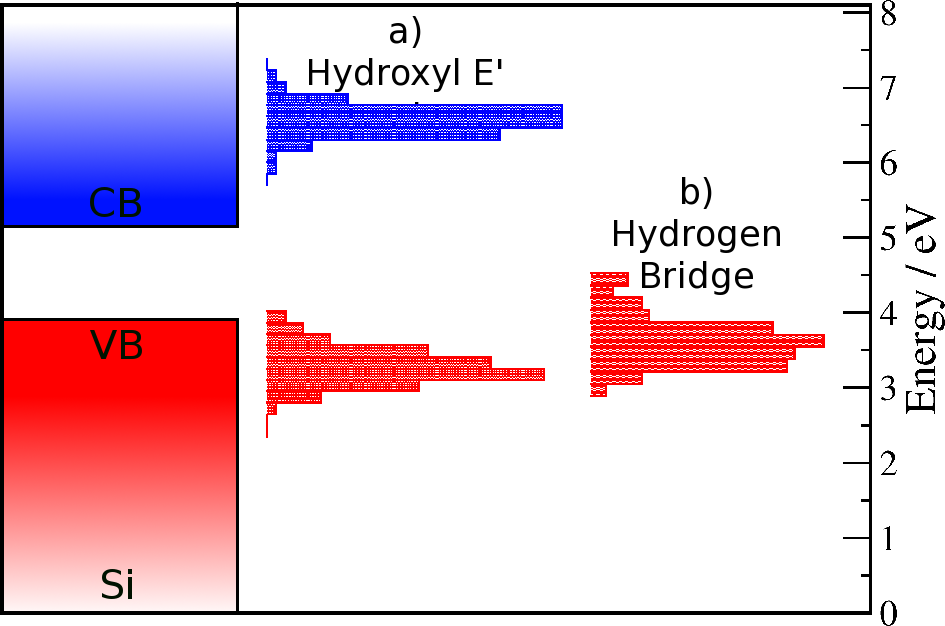
\includegraphics{hdefects_sisio2.png}
\caption{Histogram of the one-electron level of 116 configurations of; a) the hydroxyl E$^\prime$ center, b) 72 configurations of the hydrogen bridge defect. The energy scale starts from 0.0 and finishes at 8.1 eV; this is the a-SiO$_2$ band gap as calculated using the PBE0\_TC\_LRC functional. The area in the histograms colored dark red show occupied states while the area of the histograms colored blue show the unoccupied states. Note that the hydrogen bridge defect has no unoccupied states in the a-SiO$_2$ band gap. The distribution of defect levels are displayed next to a schematic of the Si band structure. The band offsets are smaller than experiment as they have been scaled by the ratio between the DFT band gap and the experimental band gap of a-SiO$_2$.} 
\label{fig:sio2_h_dos}
\end{figure}

As noted in Ref. \cite{aelsayed_prl}, the hydroxyl E$^\prime$ center can be more thermodynamically stable than the interstitial H atom and is also lower in energy than the [SiO$_4$/H]$^0$ center by 1.1 eV on average. To demonstrate that, we have calculated the formation energies of 50 configurations of the hydroxyl E$^\prime$ center and of an interstitial H atom with respect to the Fermi level of the system according to equation \ref{eq:formation_fermi}. The atomic defect configurations corresponding to the neutral, positive and negative charge states of these defects used in these calculations are shown in Fig. \ref{fig:hydroxy_thermodynamic}a. 

\begin{figure}[h!]
\includegraphics{formation_thermodynamic_levels3.png}
\caption{Formation energy of the hydroxyl E$^\prime$ center in a-SiO$_2$. a) Configurations of the hydroxyl E$^\prime$ center and interstitial hydrogen atom used in the calculations of the formation energies.  The configurations are labeled as 0, +, and - for the neutral, positive and negative charge states, respectively, with D and I standing for defect and interstitial, respectively. b) Plot of the formation energy versus the Fermi level (with respect to the a-SiO$_2$ valence band) of a single configuration of the hydroxyl E$^\prime$ center and an interstitial H atom. Formation energies corresponding to the hydroxyl E$^\prime$ center are drawn as solid red lines while the interstitial H atom's formation energies are drawn as dashed black lines.}
\label{fig:hydroxy_thermodynamic}
\end{figure}

In this figure we call the hydroxyl E$^\prime$ center and the interstitial hydrogen D and I, respectively, along with their corresponding charge of either neutral, positive or negative. The flexibility of the a-SiO$_2$ network means that both defects in the positive and negative charge states undergo large atomic relaxation with respect to the neutral state and form new configurations, which are interesting in their own rights. However, a detailed discussion on these configurations is beyond the scope of this paper. The positively charged hydroxyl E$^\prime$ center is described in more detail in Ref. \cite{h_charged_mee}. The atomic configurations of H$^+$ and H$^-$ shown in Fig. \ref{fig:hydroxy_thermodynamic}a are very close to those considered in Refs. \cite{godet_hydrogen,robertson_oxides}.

Remarkably, we find that 15 out of 50 of configurations of the hydroxyl E$^\prime$ center are thermodynamically stable in the neutral charge state over a range of Fermi levels, in contrast to what has been calculated for interstitial hydrogen in the literature.~\cite{godet_hydrogen,robertson_oxides}.  The formation energy as a function of the Fermi level position for one such configuration is shown in Fig. \ref{fig:hydroxy_thermodynamic}b). 

A histogram illustrating the distribution of thermodynamic switching levels of all 50 configurations of the hydroxyl E$^\prime$ center is shown in Fig. \ref{fig:hydroxy_thermodynamic_levels}. For the configurations in which the (+/-) switching level was lower, only this value was recorded; however, in the systems where (+/0) is lower, both the (+/0) and (0/-) levels were recorded. Together with Fig. \ref{fig:sio2_h_dos}a, the histogram shows a wide distribution of transition levels. We note that only about 30\% of all hydroxyl E$^\prime$ centers considered are thermodynamically stable at some Fermi level position and some of them have a much narrower range of stability that others. This range, however, overlaps strongly with the position of the Si band gap, indicating that hydroxyl E$^\prime$ centers can exchange electrons and holes with Si substrate. About 70\% of hydroxyl E$^\prime$ centers are negative-U centers and can exist in a-SiO$_2$ in the neutral state before trapping an electron or hole from a substrate or other defects (see e.g. discussion in Refs. \cite{shkrob1,shkrob2}).  

\begin{figure}[h!]
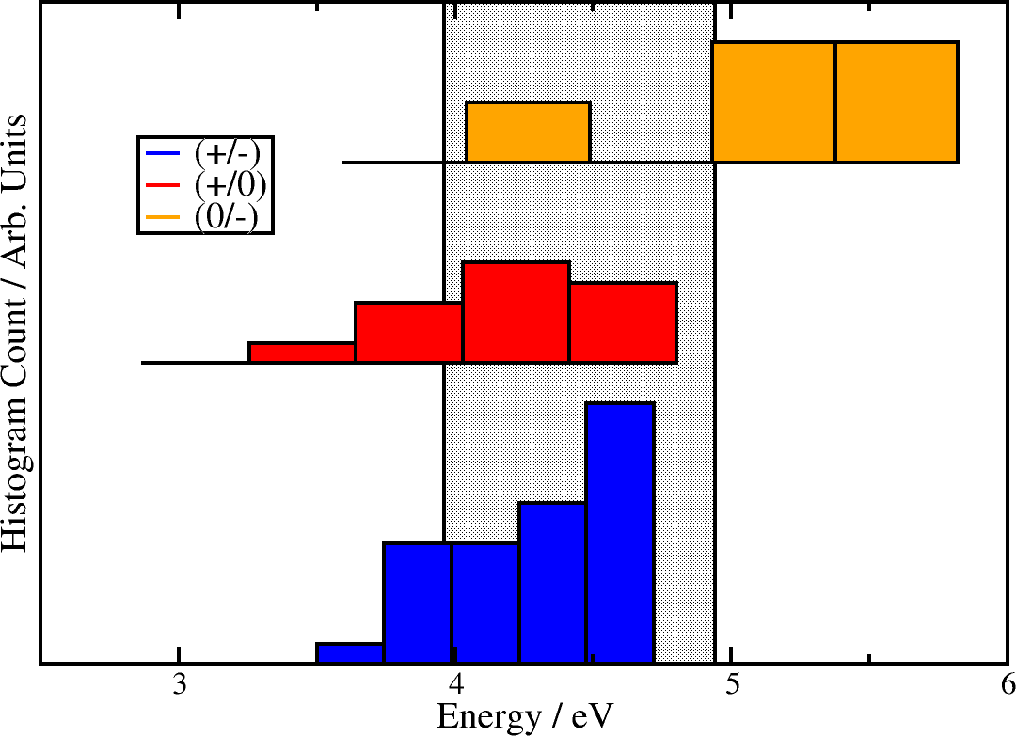
\includegraphics{thermodynamic_levels4.png}
\caption{Histogram of the thermodynamic switching levels. The (+/-) levels are recorded in the bottom histogram, the (+/0) levels in the middle and the (0/-) at the top. The position of the Si band gap is the shaded section.}
\label{fig:hydroxy_thermodynamic_levels}
\end{figure}

Barriers for transformation from an interstitial H atom into hydroxyl E$^\prime$ center configuration were calculated using the CI-NEB method in 13 different models. A schematic of this reaction is shown as Reaction 1 in Table \ref{tab:hydroxyl_barriers} along with the calculated barriers. They range over 1.0 eV due to variations in local geometry of amorphous structures, clearly emphasizing the importance of obtaining statistics when modeling amorphous SiO$_2$ and demonstrating that there are some configurations where it will be much more likely for atomic H to create this defect. We note that the distribution of calculated barriers is asymmetric and does not result in a normal distribution. This is due to the variations in the a-SiO$_2$ structures, where each local chemical environment modulates the calculated barrier, and a relatively small statistical sample.

These results demonstrate that the hydroxyl E$^\prime$ center is more thermodynamically stable than the [SiO$_4$/H]$^0$ center and has a smaller barrier to form. These two centers have different precursors (elongated and reduced \mbox{Si--O} bonds, respectively) and can be formed at different sites. However, if both centers are formed on the same SiO$_4$ tetrahedron, the barrier for transformation of the [SiO$_4$/H]$^0$ center into the hydroxyl E$^\prime$ center is only 0.1 eV.  Therefore the hydroxyl E$^\prime$ center is more likely to be formed in a-SiO$_2$ network both kinetically and thermodynamically and we will focus on the reactions of this defect in the further discussion. 

\subsubsection{Passivation and De-passivation of Hydroxyl E$^\prime$ Centers}

Hydrogen passivation of the E$^\prime$ center and 3-coordinated Si defects in a-SiO$_2$ has been studied experimentally.~\cite{fleetwood_h_device} For example, the electron spin resonance (ESR) signal of the E$^\prime$ center is significantly reduced after a soak in an ambient of H$_2$ or forming gas.~\cite{h2crack_li} We investigated the passivation and de-passivation of the hydroxyl E$^\prime$ center in the presence of both atomic and molecular hydrogen. 

The interaction of atomic H with the hydroxyl E$^\prime$ center was studied in 26 different configurations. In all cases we find that the defect is indeed passivated by H, forming a stable \mbox{Si--H} bond, which averages at 1.45 {\AA}, ranging from 1.43 {\AA} to 1.46 {\AA}. The corresponding defect level is now located at the top of the a-SiO$_2$ valence band. We calculated the binding/dissociation energy of the \mbox{Si--H} bond as:

\begin{equation}
E_{Binding}=E^{Tot}_{Interstitial}-E^{Tot}_{Si\text{--}H},
\label{eq:binding}
\end{equation}

where $E^{Tot}_{Interstitial}$ is the total energy of the system with the hydroxyl E$^\prime$ center and an interstitial H atom located far from it, $E^{Tot}_{Si\text{--}H}$ is the total energy of the system after the defect has been passivated. The geometry was fully optimized in both cases. We note that energies of the interstitial H atom in different voids in a-SiO$_2$ have a spread of about 0.2 eV. To decrease the associated uncertainty in E$_{Binding}$ we were choosing similar sites in all defect configurations. The calculated binding for the nascent \mbox{Si--H} bond is strong, averaging at 4.2 eV and ranging from 4.0 to 4.3 eV calculated from 13 systems. Reaction 2 in Table \ref{tab:hydroxyl_barriers} shows this process and the corresponding binding energies. These results confirm that the Si dangling bond passivation by atomic H is indeed very effective. 

We also investigated how the interaction of a H$_2$ molecule with a stoichiometric a-SiO$_2$ network can result in creation of a passivated defect structure discussed above without initial creation of an active defect (reaction 3 in Table \ref{tab:hydroxyl_barriers}). This reaction is thought to be responsible for hydrogen corrosion of telecom fibers. In 10 different configurations of a-SiO$_2$, H$_2$ molecules were placed in interstitial positions and their geometries were optimized. H$_2$ molecule located in the middle of an \mbox{Si--O} void interacts negligibly with the a-SiO$_2$ matrix, similar to interstitial H atoms described earlier and in good agreement with previous calculations.~\cite{BUNSON99,blochl_vacancies} Passivated defect structures were then generated by breaking a long \mbox{Si--O} bond and forming an \mbox{Si--H} bond and an \mbox{O--H} bond facing each other. After the geometry optimization we find a wide variation in the stabilities of the passivated defect structures. On average, they are by 0.2 eV more thermodynamically stable than interstitial H$_2$ molecules, ranging from being 0.61 more to 0.29 eV less stable. The barriers for this process and a reverse reaction calculated using the CI-NEB method with the interstitial H$_2$ and passivated configuration described above used as the initial and final images respectively, are presented as Reaction 3 in Table \ref{tab:hydroxyl_barriers}. The barriers for the forward reaction average at 1.74 eV while they average at 1.94 eV for the reverse reaction. The forward barrier is relatively high and would require a high temperature to overcome and form a passivated hydroxyl E$^\prime$ center, but the reverse barrier indicates that once it is formed it would remain stable.

\begin{table*}
\begin{tabular}{|l||c|c|c||c|c|c|c|}
\hline
\hline
& \multicolumn{3}{c||}{Forward Reactions} & \multicolumn{3}{|c|}{Reverse Reactions} & $\Delta$E\\
\cline{2-7}
Reaction & Min. & Max.  & Avg. & Min. & Max. & Avg. &  \\
\hline
\multicolumn{8}{|c|}{Hydrogen reactions in defect free a-SiO$_2$} \\
\hline
1) \schemestart
\setatomsep{2em}\chemfig{O_3~Si-[:30]O-[:-30]Si~O_3}\chemsign{+}\chemfig{H^0}\arrow{<->>}\setatomsep{2em}\chemfig{O_3~\lewis{0.,Si}-[1,,,,draw=none]HO-[7]Si~O_3}
\schemestop & 0.50 & 1.71  & 0.91 & 1.25 & 2.40 & 1.66 & -0.75 \\
\hline
2) \schemestart
\setatomsep{2em}\chemfig{O_3~\lewis{0.,Si}-[1,,,,draw=none]HO-[7]Si~O_3}\chemsign{+}\chemfig{H^0}\arrow{->}\setatomsep{2em}\chemfig{O_3~Si-H-[1,,,,draw=none]HO-[7]Si~O_3}
\schemestop & 0.00 & 0.00  & 0.00 & 3.96 & 4.31 & 4.19 & -4.19 \\
\hline
3) \schemestart
\setatomsep{2em}\chemfig{O_3~Si-[:30]O-[:-30]Si~O_3}\chemsign{+}\chemfig{H_2}\arrow{<->>}\setatomsep{2em}\chemfig{O_3~Si-H-[1,,,,draw=none]HO-[7]Si~O_3}
\schemestop & 1.07 & 2.15 & 1.74 & 1.57 & 2.45 & 1.94 & -0.20 \\
\hline
4) \schemestart
\setatomsep{2em}\chemfig{O_3~\lewis{0.,Si}-[1,,,,draw=none]HO-[7]Si~O_3}\chemsign{+}\chemfig{H_2}\arrow{<<->}\setatomsep{2em}\chemfig{O_3~Si-H-[1,,,,draw=none]HO-[7]Si~O_3}\chemsign{+}\chemfig{H^0}
\schemestop & 0.46 & 0.78 & 0.65 & 0.10 & 0.24 & 0.20 & 0.45\\
\hline
\multicolumn{8}{|c|}{Hydrogen reactions with an oxygen vacancy in a-SiO$_2$}\\
\hline
5) \schemestart
\setatomsep{2em}\chemfig{O_3~Si-[0,,,,draw=none]Si~O_3}\chemsign{+}\chemfig{H^0}\arrow{->}\setatomsep{2em}\chemfig{O_3~\lewis{0.,Si}-[1,,,,draw=none]H-[7]Si~O_3}
\schemestop & 0.00 & 0.00  & 0.00 & 0.16 & 4.26 & 2.76 & -2.76 \\
\hline
6) \schemestart
\setatomsep{2em}\chemfig{O_3~\lewis{0.,Si}-[1,,,,draw=none]H-[7]Si~O_3}\chemsign{+}\chemfig{H^0}\arrow{->}\setatomsep{2em}\chemfig{O_3~Si-H-[1,,,,draw=none]H-[7]Si~O_3}
\schemestop & 0.00 & 0.00  & 0.00 & 0.49 & 4.48 & 2.78 & -2.78 \\
\hline
7) \schemestart
\setatomsep{2em}\chemfig{O_3~Si-[0,,,,draw=none]Si~O_3}\chemsign{+}\chemfig{H_2}\arrow{<->>}\setatomsep{2em}\chemfig{O_3~Si-H-[1,,,,draw=none]H-[7]Si~O_3} 
\schemestop & 0.95 & 2.36  & 1.63 & 0.59 & 4.17 & 3.18 & -1.55 \\
\hline
8) \schemestart
\setatomsep{2em}\chemfig{O_3~\lewis{0.,Si}-[1,,,,draw=none]H-[7]Si~O_3}\chemsign{+}\chemfig{H_2}\arrow{<<->}\chemfig{H_2}\setatomsep{2em}\chemfig{O_3~Si-H-[1,,,,draw=none]H-[7]Si~O_3}\chemsign{+}\chemfig{H^0}
\schemestop & 0.46 & 2.03 & 1.03 & 0.01 & 0.94  & 0.50  & -0.53 \\
\hline
\hline
\end{tabular}
\caption{Hydrogen's reactions with a-SiO$_2$. The top four reactions are associated with a defect-free a-SiO$_2$ matrix and the hydroxyl E$^\prime$ center, while the bottom four reactions are associated with hydrogen's interactions with an oxygen vacancy and the hydrogen bridge defect. All results are in eV.}
\label{tab:hydroxyl_barriers}
\end{table*}

Previous theoretical studies have investigated the reaction of a H$_2$ molecule cracking at an E$^\prime$ center, passivating the defect and leaving behind an interstitial H atom.~\cite{edwards_h2,h2crack_li,h2crack_sidb_ts} This reaction has been shown to be endothermic at multiple levels of theory, i.e., the passivated configuration is thermodynamically unfavorable with respect to the active defect and an interstitial H$_2$ molecule. Our calculations for the H$_2$ reaction with the hydroxyl E$^\prime$ center (see Reaction 4 in Table \ref{tab:hydroxyl_barriers}) confirm these conclusions. The barriers calculated in 13 models are qualitatively similar to previous calculations of H$_2$ dissociation at E$^\prime$ centers,~\cite{h2crack_sidb_ts,edwards_h2,kurtz_h2} with the defect configuration in the presence of a H$_2$ molecule being thermodynamically favorable by 0.41 eV on average, ranging from 0.22 to 0.68 eV more stable. The barrier for the defect passivation by an interstitial H$_2$ molecule averages at 0.65 eV, ranging from 0.46 eV to 0.78 eV. However, the reverse barrier is much lower and averages at 0.20 eV, ranging from 0.10 eV to 0.24 eV. Similar to the \mbox{Si--H} binding energies, these barriers exhibit a much narrower range and are more resistant to fluctuations in the local environment of the a-SiO$_2$ matrix. The reverse reaction corresponds to the re-activation of the passivated hydroxyl E$^\prime$ center by an excess of H atoms. Remarkably, it suggests another channel for formation of hydroxyl E$^\prime$ centers via efficient re-activation of H passivated defects even at low temperatures. 

\subsection{Hydrogen Interaction with Oxygen Vacancies in a-SiO$_2$}
\label{sec:vacancies}

Atomic H reacts with O vacancies in SiO$_2$ creating a defect known as the hydrogen bridge.~\cite{eprime_4_1,eprime_4_2,blochl_vacancies,mysovsky_pov,VANGINHOVEN06} It was first identified in $\alpha$-quartz by Nelson \emph{et al.} using ESR,~\cite{eprime_4_2} with Isoya \emph{et al.} further resolving the signal and presenting a simple model whereby an O vacancy in quartz is decorated by a H atom.~\cite{eprime_4_1} Subsequently, Bl\"{o}chl studied the hydrogen bridge as part of his comprehensive work on hydrogen complexed defects in oxygen deficient $\alpha$-quartz.~\cite{blochl_vacancies} Using periodic models of $\alpha$-quartz, he found that a H atom would interact with an O vacancy to produce a defect state in the band gap. In the most energetically favorable state H forms one short \mbox{Si--H} bond with one of the Si atoms of the vacancy leaving the other Si atom under-coordinated. The H can be moved towards the under-coordinated Si so that a new, almost isoenergetic minimum is found where the \mbox{Si--H} bond and the under-coordinated Si are exchanged. Bl\"{o}chl used this model of the hydrogen bridge to explain stress induced leakage currents (SILC) in electronic devices that use SiO$_2$ as a gate insulator.~\cite{BLOECHL99} Mysovsky \emph{et al.} also studied the hydrogen bridge in an embedded cluster model of $\alpha$-quartz where the results agree well with Bl\"{o}chl's results.~\cite{mysovsky_pov} In this study, we investigate hydrogen's interactions with vacancies in a-SiO$_2$ using a local structure which is analogous to the hydrogen bridge structure in crystalline SiO$_2$. Due to the disordered nature of a-SiO$_2$, we have studied 144 configurations of the hydrogen bridge to obtain the necessary statistics to describe the distribution of defect's properties in a-SiO$_2$.

\begin{figure}[h!]
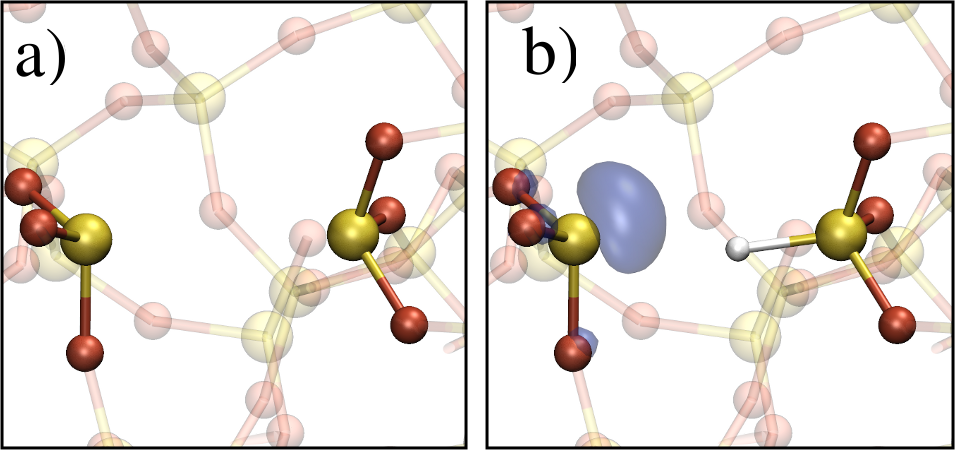
\includegraphics{hydrogen_bridge_configurations2.png}
\caption{Atomic structure and spin density of the hydrogen bridge and its precursor. Si atoms are shown in yellow, O atoms are shown in red and H atoms are shown as grey. a) Atomic structure of the oxygen vacancy which is the precursor to the hydrogen bridge. b) Atomic structure and spin density of the hydrogen bridge. The spin density is seen as the blue polyhedron.}
\label{fig:h_bridge}
\end{figure}


\subsubsection{Hydrogen Bridge Defect in a-SiO$_2$}

In order to study hydrogen's interactions with vacancies in a-SiO$_2$, all oxygen atoms in a single a-SiO$_2$ structure (generated as described in section \ref{sec:calc_details} and containing 144 O atoms) were removed one by one to create 144 configurations of the oxygen vacancy [see Fig. \ref{fig:h_bridge}a], the hydrogen bridge's precursor. A H atom was then placed by each vacancy and the geometry optimization resulted in an asymmetric defect structure, whereby the H is closer to one of the Si atoms it sits between [see Fig. \ref{fig:h_bridge}b]. This is manifested as a short \mbox{Si--H} bond and a longer \mbox{Si- -H} interaction, where \mbox{-  -} indicates a non-bonding interaction. The short \mbox{Si--H} bond averages at 1.47 {\AA} while the longer \mbox{Si-  -H} interaction averages at 2.21 {\AA}. The shorter \mbox{Si--H} bond lengths are distributed over 0.1 {\AA} while the longer \mbox{Si- -H} interaction range over 1.4 {\AA}, indicating that the shorter bond is a strong, stable interaction while the longer range \mbox{Si- -H} interaction is relatively weak and strongly influenced by the amorphous environment [see Fig. \ref{fig:hbridge_dist} for the distribution of bond lengths around the hydrogen bridge]. The \mbox{Si--O} bonds associated with both of these Si atoms average at 1.63 {\AA} and have a range of just under 0.04 {\AA}. These \mbox{Si--O} bonds are the same length as all other \mbox{Si--O} bonds in the system and this indicates that the relaxation is highly localized at the defect center. 

\begin{figure}
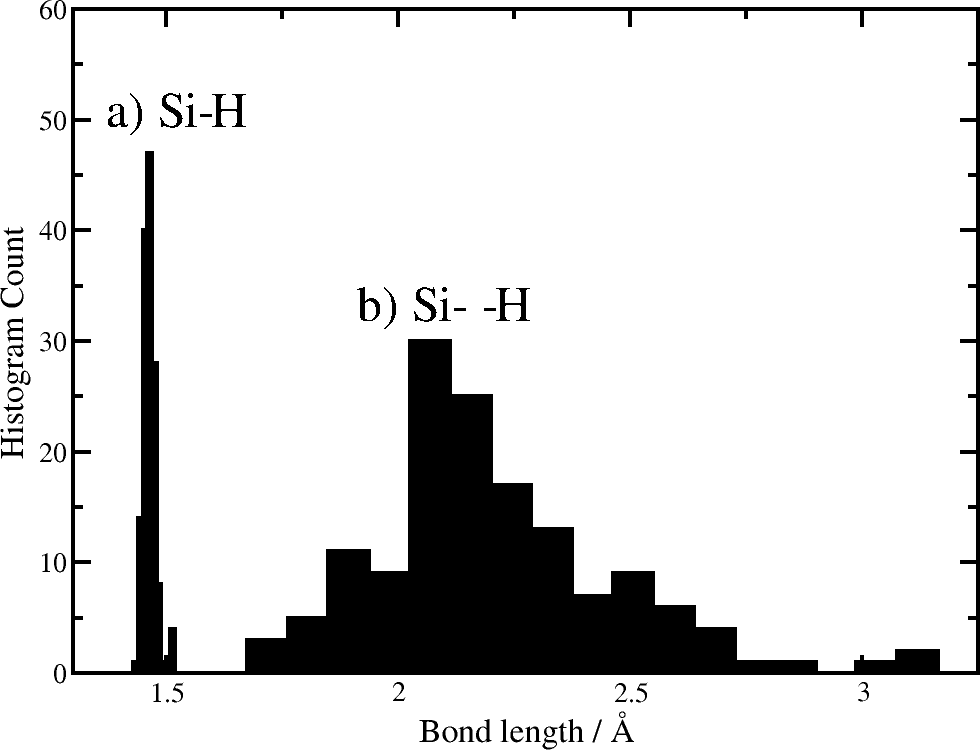
\includegraphics{hbridge_lengths_labelled.png}
\caption{Histograms of the distributions of geometries of the hydrogen bridge defect. a) Distribution of short \mbox{Si--H} bond lengths around the hydrogen bridge, shown on the right hand side of Fig. \ref{fig:h_bridge}b. b) Distribution of the longer \mbox{Si- -H} non-bonding interactions of the hydrogen bridge; i.e., the distance between the 3-coordinated Si on the left hand side of Fig. \ref{fig:h_bridge}b and the H.}
\label{fig:hbridge_dist}
\end{figure}


The formation energies of 10 hydrogen bridges and H interstitial atoms were calculated using the defect configurations shown in Fig. \ref{fig:hbridge_formation}a and the interstitial configurations shown in Fig. \ref{fig:hydroxy_thermodynamic}a. The formation energy for one of these configurations is plotted against the Fermi level in Fig. \ref{fig:hbridge_formation}b. Out of the 10 configurations, 2 show a negative-U behavior, with the remaining 8 having the neutral hydrogen bridge as the most thermodynamically stable over some range of Fermi levels. 

\begin{figure}[h!]
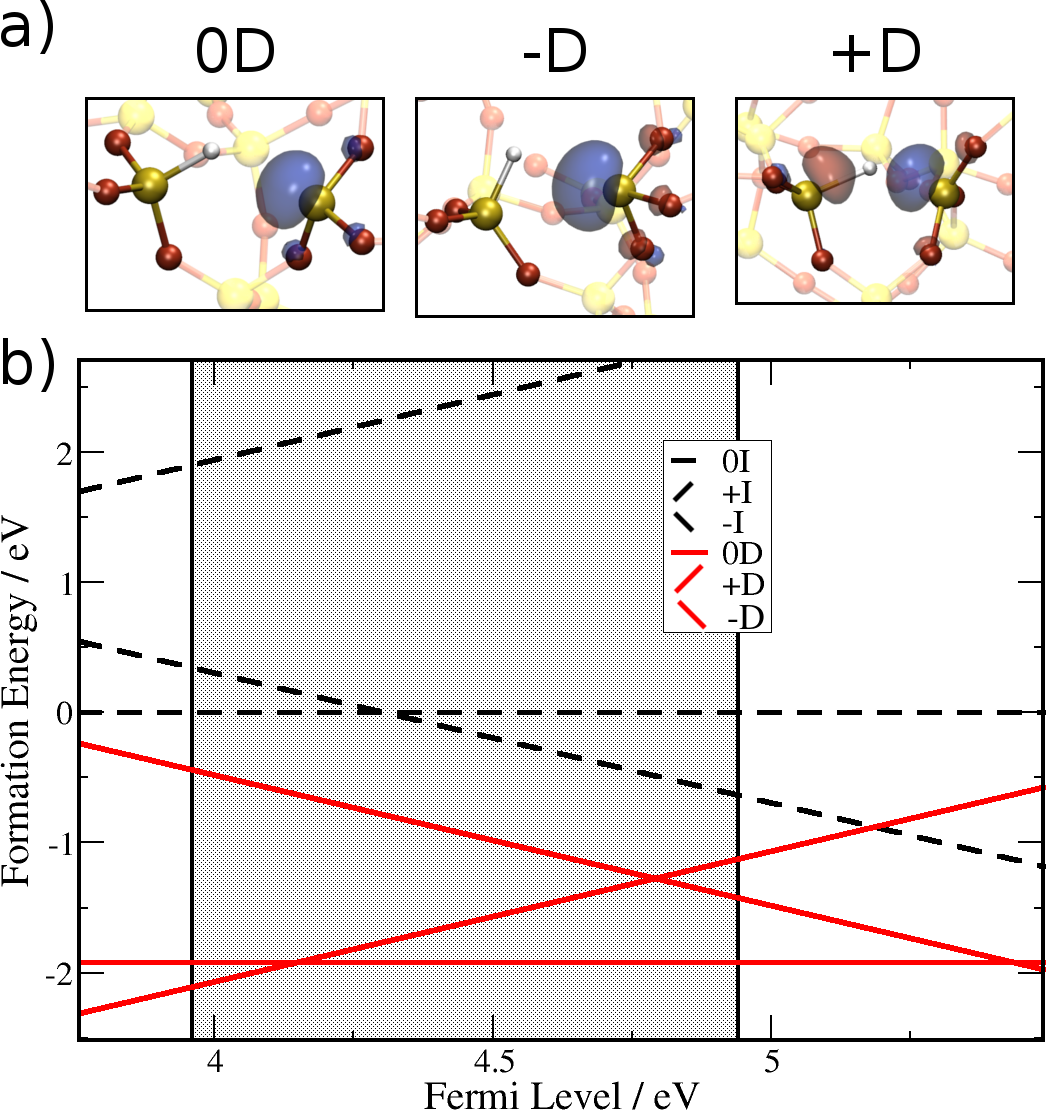
\includegraphics{hbridge_007_2.png}
\caption{Thermodynamics of the hydrogen bridge in a-SiO$_2$. The configurations are labeled as 0, +, and - for the neutral, positive and negative charge states, respectively, with D and I standing for defect and interstitial, respectively. The interstitial configurations are shown in Fig. \ref{fig:hydroxy_thermodynamic}a. a) Hydrogen bridge configurations used in the calculations of the formation energies. b) Formation energy diagram for a single configuration of the hydrogen bridge in a-SiO$_2$. The neutral hydrogen bridge (lower horizontal solid red line) is the most thermodynamically stable charge state for a single hydrogen atom in an oxygen vacancy across a range of Fermi levels.}
\label{fig:hbridge_formation}
\end{figure}


The binding energy of the \mbox{Si--H} bond of the hydrogen bridge defect was calculated as:

\begin{equation}
E_{Binding}=E^{Tot}_{O_{vac} + Interstitial}-E^{Tot}_{H-bridge},
\end{equation}

where $E^{Tot}_{O_{vac} + Interstitial}$ is the energy of an a-SiO$_2$ structure with an O vacancy and an interstitial H atom in the same periodic cell far from the defect, and $E^{Tot}_{H-bridge}$ is the total energy of the hydrogen bridge defect in the same a-SiO$_2$ system. The geometries of both systems are fully optimized. The calculated binding energies of the \mbox{Si--H} bond averages at 2.76 eV and ranges over 4 eV. Such a broad distribution of binding energies is due to the vacancy reforming an \mbox{Si--Si} bond when the H atom is moved to an interstitial position. The distribution of \mbox{Si--Si} bond lengths and energies is very wide, and the accompanying long-range network relaxation is strong and depends on the local environment of the vacancy.~\cite{asio2_3} In contrast, the geometry of the passivated hydroxyl E$^\prime$ center changes very little when the H atom is moved to an interstitial position and hence the distribution of binding energies there is much more narrow.

The electronic density of states shows a one-electron level located on average 3.7 eV above the SiO$_2$ valence band [see Fig. \ref{fig:sio2_h_dos}b]; taking the Si/SiO$_2$ valence band offset into account this defect level is almost resonant with the top of the Si valence band, similar to the hydroxyl E$^\prime$ center. Mulliken charge analysis on the H reveals that it is on average -0.21 $|e|$ and has a range of just under 0.2 $|e|$. The charge of the H shows a linear dependence on the distance between the Si dangling bond and the H, being more negatively charged the shorter the \mbox{Si- -H} interaction [see the black stars in Fig. \ref{fig:hbridge_correlation}]. The defect level position shows a strong anti-correlation to the \mbox{Si- -H} interaction, with the defect level moving closer to the SiO$_2$ valence band as the \mbox{Si- -H} distance gets longer. We attribute this to the slightly negative charge of the H which results in the defect level being pushed up when the H is closer to the localized electron. The asymmetric geometry relaxation, the position of the defect level, and the analysis of the electronic structure (see Fig. \ref{fig:h_bridge}b) indicate that the hydrogen bridge defect consists of a strong \mbox{Si--H} bond facing a Si dangling bond, analogous to the hydrogen bridge in $\alpha$-quartz. However, in the amorphous matrix there are configurations which allow the Si dangling bond to relax further, resulting in a very wide range of \mbox{Si- -H} interactions which cannot occur in $\alpha$-quartz. This interaction affects the Mulliken charges of the constituent atoms of the defect and results in a wide distribution of defect levels.

\begin{figure}[h!]
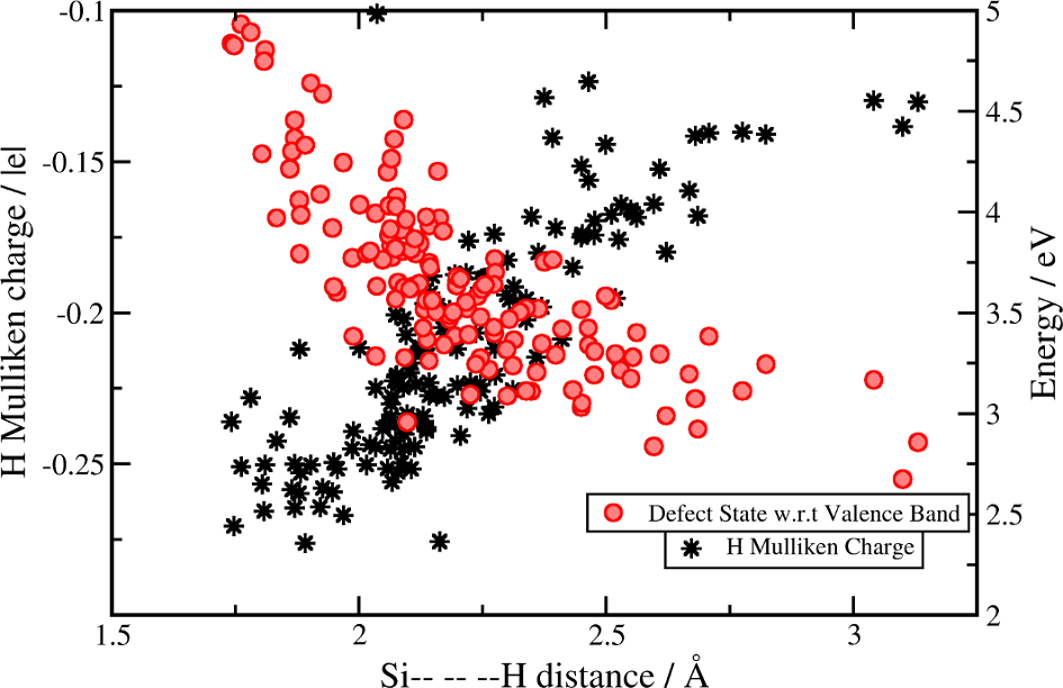
\includegraphics{hbridge_analysis.png}
\caption{Mulliken charge of H in the hydrogen bridge and the defect level plotted against the long \mbox{Si- -H} interaction. The left axis is the Mulliken charge and the black stars are the Mulliken charges of the H. The right axis is energy in eV and the red circles are the defect levels of the hydrogen bridge with respect to the top of the a-SiO$_2$ valence band.} 
\label{fig:hbridge_correlation}
\end{figure}

%\begin{figure}[h!]
%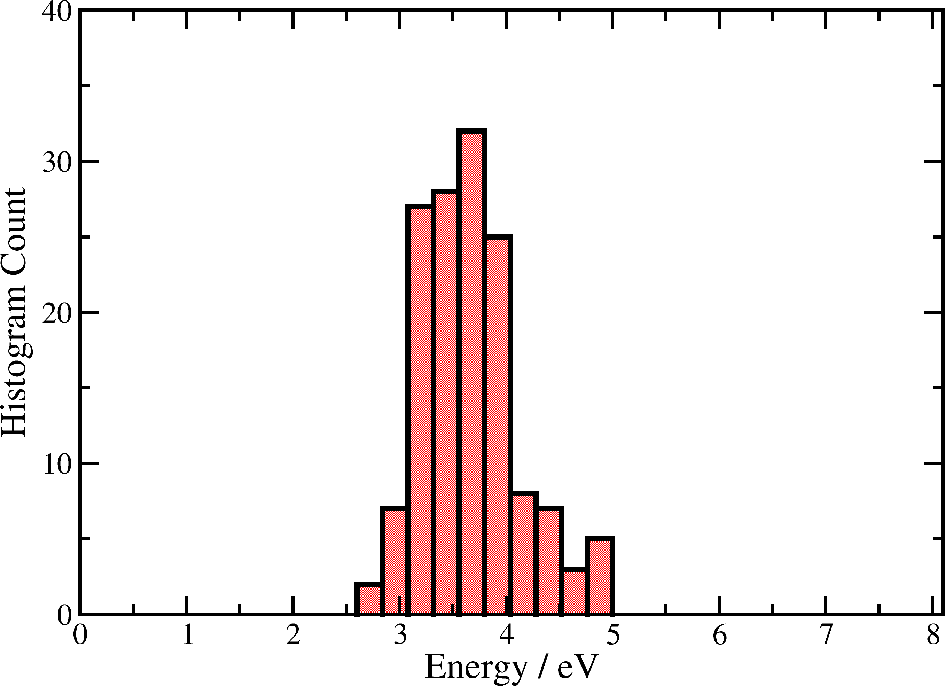
\includegraphics{hbridge_defectlevel.png}
%\caption{Histogram of the electronic density of states of 72 configurations of the hydrogen bridge defect. The energy scale starts from 0.0 and finishes at 8.1 eV; this is the a-SiO$_2$ band gap as calculated using the PBE0\_TC\_LRC functional. The area which is colored dark red and centers around 3.5 eV shows the occupied states of the hydrogen bridge defect. No unoccupied states sit in the band gap.}
%\label{fig:hbridge_defectlevel}
%end{figure}

\subsubsection{Passivation and De-passivation of Hydrogen Bridge}

The hydrogen bridge contains a Si dangling bond, which could be passivated by H atom. In 10 defect configurations, an H atom was placed close to the dangling bond and the geometries of these configurations were optimized. The resulting structures now contain two \mbox{Si--H} bonds and are summarized schematically as Reaction 6 in Table \ref{tab:hydroxyl_barriers}. Analysis of the electronic structure of these passivated configurations reveals that all defect states in the band gap are suppressed. The binding energies of the resulting \mbox{Si--H} bonds were calculated according to equation \ref{eq:binding} and by placing an interstitial H atom a few {\AA} away from the defect center, averaging at 2.8 eV and ranging over 3 eV. This average value is smaller than that for the hydroxyl E$^\prime$ center due to repulsion between the two hydrogens. The distribution is wide because of the strong structural relaxation of both defect configurations and different local environments.

We investigated how this fully passivated configuration could be generated directly as a result of a well-known reaction of a H$_2$ molecule with an O vacancy, shown schematically as Reaction 7 in Table \ref{tab:hydroxyl_barriers}. The optimized configurations of an interstitial H$_2$ molecule were calculated and used as the initial configuration for a CI-NEB calculation, while the final configurations were the passivated hydrogen bridge configurations. The barrier to H$_2$ dissociation at an O vacancy averages at 1.63 eV and ranges over 1.3 eV. The reverse reaction averages at 3.18 eV with a range of over 3.0 eV. These results show that the passivated configuration of the hydrogen bridge is very stable; however, its formation barrier from H$_2$ can be rather high and, similarly to the hydroxyl E$^\prime$ center, requires a high temperature to overcome.

Finally, we investigated whether the passivated hydrogen bridge could be de-passivated by an interstitial H in a similar manner to the hydroxyl E$^\prime$ center. This is shown schematically as Reaction 8 in Table \ref{tab:hydroxyl_barriers}. Using the passivated configuration and an interstitial H atom as the initial configuration and the active hydrogen bridge defect with an interstitial H$_2$ molecule as the final configuration, NEB calculations were run on 10 different configurations to estimate the barriers. The barrier to the forward reaction averages at 1.03 eV and exhibits a range of over 1.0 eV, while the backward reaction averages at 0.5 eV and exhibits a range of just under 1.0 eV. Again, as in the case of the hydroxyl E$^\prime$ center, the barriers for de-passivation reactions is much lower suggesting the hydrogen bridge center can be effectively re-activated in the excess of H atoms.

\section{Discussion and Conclusions}

We have studied a number of different reactions of atomic and molecular H with stoichiometric and oxygen defficient a-SiO$_2$. Our calculations show that, in contrast to previous studies,~\cite{blochl_vacancies,robertson_oxides,godet_hydrogen} neutral interstitial H atoms can interact very strongly with defect-free a-SiO$_2$ matrices, generating two different defect configurations: the [SiO$_4$/H]$^0$ and the hydroxyl E$^\prime$ center, the latter being the dominant defect. Atomic H interacts strongly with the O vacancy to produce a hydrogen bridge defect analogous to that in $\alpha$-quartz~\cite{blochl_vacancies} and characterized by an asymmetric relaxation so that a strong \mbox{Si--H} bond faces a 3-coordinated Si. Our results show a wide distribution of the hydrogen bridge defect levels, which we correlate to the Mulliken charge of the H and its distance from the 3-coordinated Si (see Fig. \ref{fig:h_bridge}). The hydroxyl E$^\prime$ and hydrogen bridge centers are both shown to have deep levels in the a-SiO$_2$ band gap, which are nearly resonant with the top of the Si valence band. Some of these defect configurations are stable in the neutral charge state over a range of Fermi level positions in the a-SiO$_2$ band gap. These results demonstrate clearly that atomic H does not act solely as a benign agent in a-SiO$_2$ at room and elevated temperatures.

Our calculations reveal that the hydroxyl E$^\prime$ and hydrogen bridge centers could have an effect on the technological applications of a-SiO$_2$. The defect levels of both defects are located close to the top of the Si valence band in a Si/SiO$_2$ system (see Fig. \ref{fig:sio2_h_dos}), typically used in metal-oxide-semiconductor (MOS) electronic devices. Holes at the top of the Si valence band, typical of a pMOS device, can tunnel into the hydroxyl E$^\prime$ and hydrogen bridge centers so that these defects can act as a source of trapped positive charge or negative bias temperature instability in such a device.

The reactions of hydrogen species with an O vacancy and with defect-free a-SiO$_2$ summarized in Table \ref{tab:hydroxyl_barriers} show qualitatively similar behavior for both defects. Our results for H$_2$ dissociation at the hydroxyl E$^\prime$ and hydrogen bridge centers can explain the slow passivation kinetics of the E$^\prime$ center signals under an H$_2$ atmosphere. The barrier to H$_2$ cracking and passivation is quite high while the final configuration is thermodynamically unfavorable in the presence of an H atom, indicating that the passivation reaction would proceed rather slowly. It is also important to note the consequence of the backwards reactions, which are essentially re-activating the passivated defect. The barriers for the de-passivation reactions are rather low and, if a source of atomic H exists in the system, it can de-passivate \mbox{Si--H} bonds and activate a hydroxyl E$^\prime$ or hydrogen bridge center. Notably, the de-passivation reactions studied are also similar to the experimentally observed de-passivation of the P$_b$ center, a defect consisting of a 3-coordinated Si with a trapped electron, which exists at the Si/SiO$_2$ interface~\cite{cartier_depassivation}. The de-passivation reaction is insensitive to how the passivated configuration was generated in the first place and is only limited by the concentration and diffusion of atomic H in the system. Atomic H has can be released into the a-SiO$_2$ layer in metal-oxide-semiconductor (MOS) devices in a number of conditions~\cite{h_gate1,h_gate2,poindexter_hydrogenous}. Coupled with the results for the de-passivation reactions and the positions of the hydroxyl E$^\prime$ and hydrogen bridge defect levels, these results strongly suggest that the hydroxyl E$^\prime$ and hydrogen bridge are potentially detrimental defects for electronic and optical technologies.

\section{Acknowledgements}
We are grateful to L. Skuja, K. Kajihara, B. Kaczer, A. Stesmans, and G. Pobegen for valuable and illuminating discussions. The authors acknowledge EPSRC and the EU FP7 project MORDRED (EU Project grant No. 261868) and COST Action CM1104 for financial support. We would like to thank the UK's HPC Materials Chemistry Consortium, which is funded by EPSRC (EP/F067496), for providing computer resources on the UK's national high-performance computing service HECToR and Archer. 

\begin{thebibliography}{80}%
\makeatletter
\providecommand \@ifxundefined [1]{%
 \@ifx{#1\undefined}
}%
\providecommand \@ifnum [1]{%
 \ifnum #1\expandafter \@firstoftwo
 \else \expandafter \@secondoftwo
 \fi
}%
\providecommand \@ifx [1]{%
 \ifx #1\expandafter \@firstoftwo
 \else \expandafter \@secondoftwo
 \fi
}%
\providecommand \natexlab [1]{#1}%
\providecommand \enquote  [1]{``#1''}%
\providecommand \bibnamefont  [1]{#1}%
\providecommand \bibfnamefont [1]{#1}%
\providecommand \citenamefont [1]{#1}%
\providecommand \href@noop [0]{\@secondoftwo}%
\providecommand \href [0]{\begingroup \@sanitize@url \@href}%
\providecommand \@href[1]{\@@startlink{#1}\@@href}%
\providecommand \@@href[1]{\endgroup#1\@@endlink}%
\providecommand \@sanitize@url [0]{\catcode `\\12\catcode `\$12\catcode
  `\&12\catcode `\#12\catcode `\^12\catcode `\_12\catcode `\%12\relax}%
\providecommand \@@startlink[1]{}%
\providecommand \@@endlink[0]{}%
\providecommand \url  [0]{\begingroup\@sanitize@url \@url }%
\providecommand \@url [1]{\endgroup\@href {#1}{\urlprefix }}%
\providecommand \urlprefix  [0]{URL }%
\providecommand \Eprint [0]{\href }%
\providecommand \doibase [0]{http://dx.doi.org/}%
\providecommand \selectlanguage [0]{\@gobble}%
\providecommand \bibinfo  [0]{\@secondoftwo}%
\providecommand \bibfield  [0]{\@secondoftwo}%
\providecommand \translation [1]{[#1]}%
\providecommand \BibitemOpen [0]{}%
\providecommand \bibitemStop [0]{}%
\providecommand \bibitemNoStop [0]{.\EOS\space}%
\providecommand \EOS [0]{\spacefactor3000\relax}%
\providecommand \BibitemShut  [1]{\csname bibitem#1\endcsname}%
\let\auto@bib@innerbib\@empty
%</preamble>
\bibitem [{\citenamefont {Lenahan}(2008)}]{LENAHAN08}%
  \BibitemOpen
  \bibfield  {author} {\bibinfo {author} {\bibfnamefont {P.}~\bibnamefont
  {Lenahan}},\ }in\ \href@noop {} {\emph {\bibinfo {booktitle} {Defects in
  Microelectronic Materials and Devices}}},\ \bibinfo {editor} {edited by\
  \bibinfo {editor} {\bibfnamefont {D.}~\bibnamefont {Fleetwood}}, \bibinfo
  {editor} {\bibfnamefont {R.}~\bibnamefont {Schrimpf}}, \ and\ \bibinfo
  {editor} {\bibfnamefont {S.}~\bibnamefont {Pantelides}}}\ (\bibinfo
  {publisher} {Taylor and Francis/CRC Press},\ \bibinfo {year} {2008})\
  \bibinfo {note} {(invited)}\BibitemShut {NoStop}%
\bibitem [{\citenamefont {Pobegen}\ \emph {et~al.}(2013)\citenamefont
  {Pobegen}, \citenamefont {Nelhiebel},\ and\ \citenamefont
  {Grasser}}]{pobegen_h}%
  \BibitemOpen
  \bibfield  {author} {\bibinfo {author} {\bibfnamefont {G.}~\bibnamefont
  {Pobegen}}, \bibinfo {author} {\bibfnamefont {M.}~\bibnamefont {Nelhiebel}},
  \ and\ \bibinfo {author} {\bibfnamefont {T.}~\bibnamefont {Grasser}},\ }in\
  \href@noop {} {\emph {\bibinfo {booktitle} {Reliability Physics Symposium
  (IRPS), 2013 IEEE International}}}\ (\bibinfo {year} {2013})\ pp.\ \bibinfo
  {pages} {XT.10.1--XT.10.6}\BibitemShut {NoStop}%
\bibitem [{\citenamefont {Cartier}\ \emph {et~al.}(1993)\citenamefont
  {Cartier}, \citenamefont {Stathis},\ and\ \citenamefont
  {Buchanan}}]{cartier_depassivation}%
  \BibitemOpen
  \bibfield  {author} {\bibinfo {author} {\bibfnamefont {E.}~\bibnamefont
  {Cartier}}, \bibinfo {author} {\bibfnamefont {J.~H.}\ \bibnamefont
  {Stathis}}, \ and\ \bibinfo {author} {\bibfnamefont {D.~A.}\ \bibnamefont
  {Buchanan}},\ }\href@noop {} {\bibfield  {journal} {\bibinfo  {journal}
  {Appl. Phys. Lett.}\ }\textbf {\bibinfo {volume} {63}},\ \bibinfo {pages}
  {1510} (\bibinfo {year} {1993})}\BibitemShut {NoStop}%
\bibitem [{\citenamefont {Stathis}\ and\ \citenamefont
  {Cartier}(1994)}]{stathis_depassivation}%
  \BibitemOpen
  \bibfield  {author} {\bibinfo {author} {\bibfnamefont {J.~H.}\ \bibnamefont
  {Stathis}}\ and\ \bibinfo {author} {\bibfnamefont {E.}~\bibnamefont
  {Cartier}},\ }\href {\doibase 10.1103/PhysRevLett.72.2745} {\bibfield
  {journal} {\bibinfo  {journal} {Phys. Rev. Lett.}\ }\textbf {\bibinfo
  {volume} {72}},\ \bibinfo {pages} {2745} (\bibinfo {year}
  {1994})}\BibitemShut {NoStop}%
\bibitem [{\citenamefont {Henschel}\ \emph {et~al.}(2002)\citenamefont
  {Henschel}, \citenamefont {Kohn},\ and\ \citenamefont
  {Weinand}}]{hydrogen_ria}%
  \BibitemOpen
  \bibfield  {author} {\bibinfo {author} {\bibfnamefont {H.}~\bibnamefont
  {Henschel}}, \bibinfo {author} {\bibfnamefont {O.}~\bibnamefont {Kohn}}, \
  and\ \bibinfo {author} {\bibfnamefont {U.}~\bibnamefont {Weinand}},\
  }\href@noop {} {\bibfield  {journal} {\bibinfo  {journal} {IEEE Trans. Nucl.
  Sci.}\ }\textbf {\bibinfo {volume} {49}},\ \bibinfo {pages} {1401} (\bibinfo
  {year} {2002})}\BibitemShut {NoStop}%
\bibitem [{\citenamefont {Suñé}\ and\ \citenamefont
  {Wu}(2002)}]{hydrogen_breakdown}%
  \BibitemOpen
  \bibfield  {author} {\bibinfo {author} {\bibfnamefont {J.}~\bibnamefont
  {Suñé}}\ and\ \bibinfo {author} {\bibfnamefont {E.}~\bibnamefont {Wu}},\
  }\href@noop {} {\bibfield  {journal} {\bibinfo  {journal} {Solid-State
  Electronics}\ }\textbf {\bibinfo {volume} {46}},\ \bibinfo {pages} {1825 }
  (\bibinfo {year} {2002})}\BibitemShut {NoStop}%
\bibitem [{\citenamefont {Hobbs}(1985)}]{hobbs_h}%
  \BibitemOpen
  \bibfield  {author} {\bibinfo {author} {\bibfnamefont {B.~E.}\ \bibnamefont
  {Hobbs}},\ }\enquote {\bibinfo {title} {Point defects in minerals},}\ \
  (\bibinfo  {publisher} {American Geophysical Union},\ \bibinfo {year}
  {1985})\ pp.\ \bibinfo {pages} {151--169}\BibitemShut {NoStop}%
\bibitem [{\citenamefont {Griscom}(1990)}]{griscom_fibers}%
  \BibitemOpen
  \bibfield  {author} {\bibinfo {author} {\bibfnamefont {D.~L.}\ \bibnamefont
  {Griscom}},\ }\href@noop {} {\bibfield  {journal} {\bibinfo  {journal} {Nucl.
  Instr. Methods B}\ }\textbf {\bibinfo {volume} {46}},\ \bibinfo {pages} {12}
  (\bibinfo {year} {1990})}\BibitemShut {NoStop}%
\bibitem [{\citenamefont {Revesz}(1977)}]{revesz}%
  \BibitemOpen
  \bibfield  {author} {\bibinfo {author} {\bibfnamefont {A.~G.}\ \bibnamefont
  {Revesz}},\ }\href@noop {} {\bibfield  {journal} {\bibinfo  {journal} {IEEE
  Trans. Nucl. Sci.}\ }\textbf {\bibinfo {volume} {24}},\ \bibinfo {pages}
  {2102} (\bibinfo {year} {1977})}\BibitemShut {NoStop}%
\bibitem [{\citenamefont {McLean}(1980)}]{mclean_radiation}%
  \BibitemOpen
  \bibfield  {author} {\bibinfo {author} {\bibfnamefont {F.~B.}\ \bibnamefont
  {McLean}},\ }\href@noop {} {\bibfield  {journal} {\bibinfo  {journal} {IEEE
  Trans. Nucl. Sci.}\ }\textbf {\bibinfo {volume} {27}},\ \bibinfo {pages}
  {1651} (\bibinfo {year} {1980})}\BibitemShut {NoStop}%
\bibitem [{\citenamefont {Griscom}(1985{\natexlab{a}})}]{griscom_radiation1}%
  \BibitemOpen
  \bibfield  {author} {\bibinfo {author} {\bibfnamefont {D.~L.}\ \bibnamefont
  {Griscom}},\ }\href {\doibase 10.1063/1.335931} {\bibfield  {journal}
  {\bibinfo  {journal} {J. Appl. Phys.}\ }\textbf {\bibinfo {volume} {58}},\
  \bibinfo {pages} {2524} (\bibinfo {year} {1985}{\natexlab{a}})}\BibitemShut
  {NoStop}%
\bibitem [{\citenamefont {DiMaria}\ \emph {et~al.}(1993)\citenamefont
  {DiMaria}, \citenamefont {Cartier},\ and\ \citenamefont
  {Arnold}}]{dimaria_injection}%
  \BibitemOpen
  \bibfield  {author} {\bibinfo {author} {\bibfnamefont {D.~J.}\ \bibnamefont
  {DiMaria}}, \bibinfo {author} {\bibfnamefont {E.}~\bibnamefont {Cartier}}, \
  and\ \bibinfo {author} {\bibfnamefont {D.}~\bibnamefont {Arnold}},\
  }\href@noop {} {\bibfield  {journal} {\bibinfo  {journal} {J. Appl. Phys.}\
  }\textbf {\bibinfo {volume} {73}},\ \bibinfo {pages} {3367} (\bibinfo {year}
  {1993})}\BibitemShut {NoStop}%
\bibitem [{\citenamefont {Helms}\ and\ \citenamefont
  {Poindexter}(1994)}]{helms_bti}%
  \BibitemOpen
  \bibfield  {author} {\bibinfo {author} {\bibfnamefont {C.~R.}\ \bibnamefont
  {Helms}}\ and\ \bibinfo {author} {\bibfnamefont {E.~H.}\ \bibnamefont
  {Poindexter}},\ }\href@noop {} {\bibfield  {journal} {\bibinfo  {journal}
  {Rep. Prog. Phys.}\ }\textbf {\bibinfo {volume} {57}},\ \bibinfo {pages}
  {791} (\bibinfo {year} {1994})}\BibitemShut {NoStop}%
\bibitem [{\citenamefont {Pobegen}\ \emph {et~al.}(2014)\citenamefont
  {Pobegen}, \citenamefont {Aichinger},\ and\ \citenamefont
  {Nelhiebel}}]{pobegen_h_nbti}%
  \BibitemOpen
  \bibfield  {author} {\bibinfo {author} {\bibfnamefont {G.}~\bibnamefont
  {Pobegen}}, \bibinfo {author} {\bibfnamefont {T.}~\bibnamefont {Aichinger}},
  \ and\ \bibinfo {author} {\bibfnamefont {M.}~\bibnamefont {Nelhiebel}},\
  }\enquote {\bibinfo {title} {Impact of hydrogen on the bias temperature
  instability},}\ in\ \href@noop {} {\emph {\bibinfo {booktitle} {Bias
  Temperature Instability for Devices and Circuits}}},\ \bibinfo {editor}
  {edited by\ \bibinfo {editor} {\bibfnamefont {T.}~\bibnamefont {Grasser}}}\
  (\bibinfo  {publisher} {Springer},\ \bibinfo {year} {2014})\ pp.\ \bibinfo
  {pages} {485--506}\BibitemShut {NoStop}%
\bibitem [{\citenamefont {Isoya}\ \emph {et~al.}(1981)\citenamefont {Isoya},
  \citenamefont {Weil},\ and\ \citenamefont {Halliburton}}]{eprime_4_1}%
  \BibitemOpen
  \bibfield  {author} {\bibinfo {author} {\bibfnamefont {J.}~\bibnamefont
  {Isoya}}, \bibinfo {author} {\bibfnamefont {J.~A.}\ \bibnamefont {Weil}}, \
  and\ \bibinfo {author} {\bibfnamefont {L.~E.}\ \bibnamefont {Halliburton}},\
  }\href@noop {} {\bibfield  {journal} {\bibinfo  {journal} {J. Chem. Phys.}\
  }\textbf {\bibinfo {volume} {74}},\ \bibinfo {pages} {5436} (\bibinfo {year}
  {1981})}\BibitemShut {NoStop}%
\bibitem [{\citenamefont {Weeks}\ and\ \citenamefont
  {Nelson}(1960)}]{eprime_4_2}%
  \BibitemOpen
  \bibfield  {author} {\bibinfo {author} {\bibfnamefont {R.~A.}\ \bibnamefont
  {Weeks}}\ and\ \bibinfo {author} {\bibfnamefont {C.~M.}\ \bibnamefont
  {Nelson}},\ }\href@noop {} {\bibfield  {journal} {\bibinfo  {journal} {J. Am.
  Ceram. Soc.}\ }\textbf {\bibinfo {volume} {43}},\ \bibinfo {pages} {399}
  (\bibinfo {year} {1960})}\BibitemShut {NoStop}%
\bibitem [{\citenamefont {Conley}\ and\ \citenamefont
  {Lenahan}(1992)}]{CONLEY92}%
  \BibitemOpen
  \bibfield  {author} {\bibinfo {author} {\bibfnamefont {J.}~\bibnamefont
  {Conley}}\ and\ \bibinfo {author} {\bibfnamefont {P.}~\bibnamefont
  {Lenahan}},\ }\href@noop {} {\bibfield  {journal} {\bibinfo  {journal} {IEEE
  Trans.Nucl.Sci.}\ }\textbf {\bibinfo {volume} {39}},\ \bibinfo {pages} {2186}
  (\bibinfo {year} {1992})}\BibitemShut {NoStop}%
\bibitem [{\citenamefont {Li}\ \emph {et~al.}(1995)\citenamefont {Li},
  \citenamefont {Kannan}, \citenamefont {Lehman},\ and\ \citenamefont
  {Sigel}}]{kannan_hydrogen_epr}%
  \BibitemOpen
  \bibfield  {author} {\bibinfo {author} {\bibfnamefont {J.}~\bibnamefont
  {Li}}, \bibinfo {author} {\bibfnamefont {S.}~\bibnamefont {Kannan}}, \bibinfo
  {author} {\bibfnamefont {R.~L.}\ \bibnamefont {Lehman}}, \ and\ \bibinfo
  {author} {\bibfnamefont {G.~H.}\ \bibnamefont {Sigel}},\ }\href@noop {}
  {\bibfield  {journal} {\bibinfo  {journal} {Applied Physics Letters}\
  }\textbf {\bibinfo {volume} {66}},\ \bibinfo {pages} {2816} (\bibinfo {year}
  {1995})}\BibitemShut {NoStop}%
\bibitem [{\citenamefont {Girard}\ \emph {et~al.}(2013)\citenamefont {Girard},
  \citenamefont {Kuhnhenn}, \citenamefont {Gusarov}, \citenamefont {Brichard},
  \citenamefont {Van~Uffelen}, \citenamefont {Ouerdane}, \citenamefont
  {Boukenter},\ and\ \citenamefont {Marcandella}}]{girard_sio2_review}%
  \BibitemOpen
  \bibfield  {author} {\bibinfo {author} {\bibfnamefont {S.}~\bibnamefont
  {Girard}}, \bibinfo {author} {\bibfnamefont {J.}~\bibnamefont {Kuhnhenn}},
  \bibinfo {author} {\bibfnamefont {A.}~\bibnamefont {Gusarov}}, \bibinfo
  {author} {\bibfnamefont {B.}~\bibnamefont {Brichard}}, \bibinfo {author}
  {\bibfnamefont {M.}~\bibnamefont {Van~Uffelen}}, \bibinfo {author}
  {\bibfnamefont {Y.}~\bibnamefont {Ouerdane}}, \bibinfo {author}
  {\bibfnamefont {A.}~\bibnamefont {Boukenter}}, \ and\ \bibinfo {author}
  {\bibfnamefont {C.}~\bibnamefont {Marcandella}},\ }\href@noop {} {\bibfield
  {journal} {\bibinfo  {journal} {IEEE Trans. Nucl. Sci.}\ }\textbf {\bibinfo
  {volume} {60}},\ \bibinfo {pages} {2015} (\bibinfo {year}
  {2013})}\BibitemShut {NoStop}%
\bibitem [{\citenamefont {Shkrob}\ \emph {et~al.}(1999)\citenamefont {Shkrob},
  \citenamefont {Tadjikov}, \citenamefont {Chemerisov},\ and\ \citenamefont
  {Trifunac}}]{shkrob1}%
  \BibitemOpen
  \bibfield  {author} {\bibinfo {author} {\bibfnamefont {I.~A.}\ \bibnamefont
  {Shkrob}}, \bibinfo {author} {\bibfnamefont {B.~M.}\ \bibnamefont
  {Tadjikov}}, \bibinfo {author} {\bibfnamefont {S.~D.}\ \bibnamefont
  {Chemerisov}}, \ and\ \bibinfo {author} {\bibfnamefont {A.~D.}\ \bibnamefont
  {Trifunac}},\ }\href@noop {} {\bibfield  {journal} {\bibinfo  {journal} {J.
  Chem. Phys.}\ }\textbf {\bibinfo {volume} {111}},\ \bibinfo {pages} {5124}
  (\bibinfo {year} {1999})}\BibitemShut {NoStop}%
\bibitem [{\citenamefont {Shkrob}\ and\ \citenamefont
  {Trifunac}(1997)}]{shkrob2}%
  \BibitemOpen
  \bibfield  {author} {\bibinfo {author} {\bibfnamefont {I.~A.}\ \bibnamefont
  {Shkrob}}\ and\ \bibinfo {author} {\bibfnamefont {A.~D.}\ \bibnamefont
  {Trifunac}},\ }\href@noop {} {\bibfield  {journal} {\bibinfo  {journal} {J.
  Chem. Phys.}\ }\textbf {\bibinfo {volume} {107}},\ \bibinfo {pages} {2374}
  (\bibinfo {year} {1997})}\BibitemShut {NoStop}%
\bibitem [{\citenamefont {Skuja}\ \emph {et~al.}(2006)\citenamefont {Skuja},
  \citenamefont {Kajihara}, \citenamefont {Hirano}, \citenamefont {Saitoh},\
  and\ \citenamefont {Hosono}}]{skuja_hydrogen}%
  \BibitemOpen
  \bibfield  {author} {\bibinfo {author} {\bibfnamefont {L.}~\bibnamefont
  {Skuja}}, \bibinfo {author} {\bibfnamefont {K.}~\bibnamefont {Kajihara}},
  \bibinfo {author} {\bibfnamefont {M.}~\bibnamefont {Hirano}}, \bibinfo
  {author} {\bibfnamefont {A.}~\bibnamefont {Saitoh}}, \ and\ \bibinfo {author}
  {\bibfnamefont {H.}~\bibnamefont {Hosono}},\ }\href@noop {} {\bibfield
  {journal} {\bibinfo  {journal} {J. Non-cryst. Sol.}\ }\textbf {\bibinfo
  {volume} {352}},\ \bibinfo {pages} {2297} (\bibinfo {year}
  {2006})}\BibitemShut {NoStop}%
\bibitem [{\citenamefont {Skuja}\ \emph {et~al.}(2008)\citenamefont {Skuja},
  \citenamefont {Kajihara},\ and\ \citenamefont {Hirano}}]{skuja_hydrogen2}%
  \BibitemOpen
  \bibfield  {author} {\bibinfo {author} {\bibfnamefont {L.}~\bibnamefont
  {Skuja}}, \bibinfo {author} {\bibfnamefont {K.}~\bibnamefont {Kajihara}}, \
  and\ \bibinfo {author} {\bibfnamefont {H.}~\bibnamefont {Hirano},
  \bibfnamefont {M.~andHosono}},\ }\href@noop {} {\bibfield  {journal}
  {\bibinfo  {journal} {Nucl. Instr. and Meth. in Phys. Res. B}\ }\textbf
  {\bibinfo {volume} {266}},\ \bibinfo {pages} {2971} (\bibinfo {year}
  {2008})}\BibitemShut {NoStop}%
\bibitem [{\citenamefont {Kajihara}\ \emph {et~al.}(2002)\citenamefont
  {Kajihara}, \citenamefont {Skuja}, \citenamefont {Hirano},\ and\
  \citenamefont {Hosono}}]{skuja_hdiffusion}%
  \BibitemOpen
  \bibfield  {author} {\bibinfo {author} {\bibfnamefont {K.}~\bibnamefont
  {Kajihara}}, \bibinfo {author} {\bibfnamefont {L.}~\bibnamefont {Skuja}},
  \bibinfo {author} {\bibfnamefont {M.}~\bibnamefont {Hirano}}, \ and\ \bibinfo
  {author} {\bibfnamefont {H.}~\bibnamefont {Hosono}},\ }\href@noop {}
  {\bibfield  {journal} {\bibinfo  {journal} {Phys. Rev. Lett.}\ }\textbf
  {\bibinfo {volume} {89}},\ \bibinfo {pages} {135507} (\bibinfo {year}
  {2002})}\BibitemShut {NoStop}%
\bibitem [{\citenamefont {Kajihara}\ \emph {et~al.}(2006)\citenamefont
  {Kajihara}, \citenamefont {Skuja}, \citenamefont {Hirano},\ and\
  \citenamefont {Hosono}}]{kajihara_hydrogen}%
  \BibitemOpen
  \bibfield  {author} {\bibinfo {author} {\bibfnamefont {K.}~\bibnamefont
  {Kajihara}}, \bibinfo {author} {\bibfnamefont {L.}~\bibnamefont {Skuja}},
  \bibinfo {author} {\bibfnamefont {M.}~\bibnamefont {Hirano}}, \ and\ \bibinfo
  {author} {\bibfnamefont {H.}~\bibnamefont {Hosono}},\ }\href@noop {}
  {\bibfield  {journal} {\bibinfo  {journal} {Phys. Rev. B}\ }\textbf {\bibinfo
  {volume} {74}},\ \bibinfo {pages} {094202} (\bibinfo {year}
  {2006})}\BibitemShut {NoStop}%
\bibitem [{\citenamefont {Vitko}(1978)}]{vitko_hydrogen}%
  \BibitemOpen
  \bibfield  {author} {\bibinfo {author} {\bibfnamefont {J.}~\bibnamefont
  {Vitko}},\ }\href@noop {} {\bibfield  {journal} {\bibinfo  {journal} {J.
  Appl. Phys.}\ }\textbf {\bibinfo {volume} {49}},\ \bibinfo {pages} {5530}
  (\bibinfo {year} {1978})}\BibitemShut {NoStop}%
\bibitem [{\citenamefont {Radzig}(1979)}]{radzig_surface}%
  \BibitemOpen
  \bibfield  {author} {\bibinfo {author} {\bibfnamefont {V.~A.}\ \bibnamefont
  {Radzig}},\ }\href@noop {} {\bibfield  {journal} {\bibinfo  {journal}
  {Kinetika i Kataliz}\ }\textbf {\bibinfo {volume} {20}},\ \bibinfo {pages}
  {456} (\bibinfo {year} {1979})}\BibitemShut {NoStop}%
\bibitem [{\citenamefont {Wilde}\ \emph {et~al.}(2002)\citenamefont {Wilde},
  \citenamefont {Matsumoto},\ and\ \citenamefont {Fukutani}}]{wilde_hdefects2}%
  \BibitemOpen
  \bibfield  {author} {\bibinfo {author} {\bibfnamefont {M.}~\bibnamefont
  {Wilde}}, \bibinfo {author} {\bibfnamefont {M.}~\bibnamefont {Matsumoto}}, \
  and\ \bibinfo {author} {\bibfnamefont {K.}~\bibnamefont {Fukutani}},\
  }\href@noop {} {\bibfield  {journal} {\bibinfo  {journal} {J. Appl. Phys.}\
  }\textbf {\bibinfo {volume} {92}},\ \bibinfo {pages} {4320} (\bibinfo {year}
  {2002})}\BibitemShut {NoStop}%
\bibitem [{\citenamefont {Afanas'ev}\ \emph {et~al.}(1995)\citenamefont
  {Afanas'ev}, \citenamefont {de~Nijs}, \citenamefont {Balk},\ and\
  \citenamefont {Stesmans}}]{asio2_hetrap3}%
  \BibitemOpen
  \bibfield  {author} {\bibinfo {author} {\bibfnamefont {V.~V.}\ \bibnamefont
  {Afanas'ev}}, \bibinfo {author} {\bibfnamefont {J.~M.~M.}\ \bibnamefont
  {de~Nijs}}, \bibinfo {author} {\bibfnamefont {P.}~\bibnamefont {Balk}}, \
  and\ \bibinfo {author} {\bibfnamefont {A.}~\bibnamefont {Stesmans}},\ }\href
  {\doibase 10.1063/1.360534} {\bibfield  {journal} {\bibinfo  {journal} {J.
  Appl. Phys.}\ }\textbf {\bibinfo {volume} {78}},\ \bibinfo {pages} {6481}
  (\bibinfo {year} {1995})}\BibitemShut {NoStop}%
\bibitem [{\citenamefont {Stesmans}\ and\ \citenamefont
  {Afanas'ev}(1998)}]{stesmans_etrap}%
  \BibitemOpen
  \bibfield  {author} {\bibinfo {author} {\bibfnamefont {A.}~\bibnamefont
  {Stesmans}}\ and\ \bibinfo {author} {\bibfnamefont {V.~V.}\ \bibnamefont
  {Afanas'ev}},\ }\href@noop {} {\bibfield  {journal} {\bibinfo  {journal}
  {Appl. Phys. Lett.}\ }\textbf {\bibinfo {volume} {72}},\ \bibinfo {pages}
  {2271} (\bibinfo {year} {1998})}\BibitemShut {NoStop}%
\bibitem [{\citenamefont {Afanas'ev}\ and\ \citenamefont
  {Stesmans}(2001{\natexlab{a}})}]{afanasev_pb}%
  \BibitemOpen
  \bibfield  {author} {\bibinfo {author} {\bibfnamefont {V.~V.}\ \bibnamefont
  {Afanas'ev}}\ and\ \bibinfo {author} {\bibfnamefont {A.}~\bibnamefont
  {Stesmans}},\ }\href@noop {} {\bibfield  {journal} {\bibinfo  {journal} {J.
  Electrochem. Soc.}\ }\textbf {\bibinfo {volume} {148}},\ \bibinfo {pages}
  {G279} (\bibinfo {year} {2001}{\natexlab{a}})}\BibitemShut {NoStop}%
\bibitem [{\citenamefont {Rivera}\ \emph {et~al.}(2002)\citenamefont {Rivera},
  \citenamefont {van Veen}, \citenamefont {Schut}, \citenamefont {de~Nijs},\
  and\ \citenamefont {Balk}}]{rivera_hdefect}%
  \BibitemOpen
  \bibfield  {author} {\bibinfo {author} {\bibfnamefont {A.}~\bibnamefont
  {Rivera}}, \bibinfo {author} {\bibfnamefont {A.}~\bibnamefont {van Veen}},
  \bibinfo {author} {\bibfnamefont {H.}~\bibnamefont {Schut}}, \bibinfo
  {author} {\bibfnamefont {J.~M.~M.}\ \bibnamefont {de~Nijs}}, \ and\ \bibinfo
  {author} {\bibfnamefont {P.}~\bibnamefont {Balk}},\ }\href@noop {} {\bibfield
   {journal} {\bibinfo  {journal} {Solid State Electron.}\ }\textbf {\bibinfo
  {volume} {46}},\ \bibinfo {pages} {1775} (\bibinfo {year}
  {2002})}\BibitemShut {NoStop}%
\bibitem [{\citenamefont {Wilde}\ and\ \citenamefont
  {Fukutani}(2014)}]{wilde_hdefect}%
  \BibitemOpen
  \bibfield  {author} {\bibinfo {author} {\bibfnamefont {M.}~\bibnamefont
  {Wilde}}\ and\ \bibinfo {author} {\bibfnamefont {K.}~\bibnamefont
  {Fukutani}},\ }\href@noop {} {\bibfield  {journal} {\bibinfo  {journal}
  {Surface Sci. Reports}\ }\textbf {\bibinfo {volume} {69}},\ \bibinfo {pages}
  {196} (\bibinfo {year} {2014})}\BibitemShut {NoStop}%
\bibitem [{\citenamefont {Afanas'ev}\ and\ \citenamefont
  {Stesmans}(1999)}]{afanasev_prb}%
  \BibitemOpen
  \bibfield  {author} {\bibinfo {author} {\bibfnamefont {V.~V.}\ \bibnamefont
  {Afanas'ev}}\ and\ \bibinfo {author} {\bibfnamefont {A.}~\bibnamefont
  {Stesmans}},\ }\href@noop {} {\bibfield  {journal} {\bibinfo  {journal}
  {Phys. Rev. B}\ }\textbf {\bibinfo {volume} {60}},\ \bibinfo {pages} {5506}
  (\bibinfo {year} {1999})}\BibitemShut {NoStop}%
\bibitem [{\citenamefont {Afanas'ev}\ \emph {et~al.}(2002)\citenamefont
  {Afanas'ev}, \citenamefont {Ciobanu}, \citenamefont {Pensl},\ and\
  \citenamefont {Stesmans}}]{afanasev_protonic1}%
  \BibitemOpen
  \bibfield  {author} {\bibinfo {author} {\bibfnamefont {V.~V.}\ \bibnamefont
  {Afanas'ev}}, \bibinfo {author} {\bibfnamefont {F.}~\bibnamefont {Ciobanu}},
  \bibinfo {author} {\bibfnamefont {G.}~\bibnamefont {Pensl}}, \ and\ \bibinfo
  {author} {\bibfnamefont {A.}~\bibnamefont {Stesmans}},\ }\href@noop {}
  {\bibfield  {journal} {\bibinfo  {journal} {Solid State Electron.}\ }\textbf
  {\bibinfo {volume} {46}},\ \bibinfo {pages} {1815} (\bibinfo {year}
  {2002})}\BibitemShut {NoStop}%
\bibitem [{\citenamefont {Afanas'ev}\ and\ \citenamefont
  {Stesmans}(2001{\natexlab{b}})}]{AFANASEV01B}%
  \BibitemOpen
  \bibfield  {author} {\bibinfo {author} {\bibfnamefont {V.}~\bibnamefont
  {Afanas'ev}}\ and\ \bibinfo {author} {\bibfnamefont {A.}~\bibnamefont
  {Stesmans}},\ }\href@noop {} {\bibfield  {journal} {\bibinfo  {journal}
  {EuroPhys.Lett.}\ }\textbf {\bibinfo {volume} {53}},\ \bibinfo {pages} {233}
  (\bibinfo {year} {2001}{\natexlab{b}})}\BibitemShut {NoStop}%
\bibitem [{\citenamefont {Afanas'ev}\ and\ \citenamefont
  {Stesmans}(1997)}]{etrapping_1}%
  \BibitemOpen
  \bibfield  {author} {\bibinfo {author} {\bibfnamefont {V.~V.}\ \bibnamefont
  {Afanas'ev}}\ and\ \bibinfo {author} {\bibfnamefont {A.}~\bibnamefont
  {Stesmans}},\ }\href@noop {} {\bibfield  {journal} {\bibinfo  {journal}
  {Phys. Rev. Lett.}\ }\textbf {\bibinfo {volume} {78}},\ \bibinfo {pages}
  {2437} (\bibinfo {year} {1997})}\BibitemShut {NoStop}%
\bibitem [{\citenamefont {Bl\"ochl}(2000)}]{blochl_vacancies}%
  \BibitemOpen
  \bibfield  {author} {\bibinfo {author} {\bibfnamefont {P. E.}~\bibnamefont
  {Bl\"ochl}},\ }\href@noop {} {\bibfield  {journal} {\bibinfo  {journal}
  {Phys. Rev. B}\ }\textbf {\bibinfo {volume} {62}},\ \bibinfo {pages} {6158}
  (\bibinfo {year} {2000})}\BibitemShut {NoStop}%
\bibitem [{\citenamefont {Yokozawa}\ and\ \citenamefont
  {Miyamoto}(1997)}]{yokozawa_h}%
  \BibitemOpen
  \bibfield  {author} {\bibinfo {author} {\bibfnamefont {A.}~\bibnamefont
  {Yokozawa}}\ and\ \bibinfo {author} {\bibfnamefont {Y.}~\bibnamefont
  {Miyamoto}},\ }\href {\doibase 10.1103/PhysRevB.55.13783} {\bibfield
  {journal} {\bibinfo  {journal} {Phys. Rev. B}\ }\textbf {\bibinfo {volume}
  {55}},\ \bibinfo {pages} {13783} (\bibinfo {year} {1997})}\BibitemShut
  {NoStop}%
\bibitem [{\citenamefont {Godet}\ and\ \citenamefont
  {Pasquarello}(2005)}]{godet_hydrogen}%
  \BibitemOpen
  \bibfield  {author} {\bibinfo {author} {\bibfnamefont {J.}~\bibnamefont
  {Godet}}\ and\ \bibinfo {author} {\bibfnamefont {A.}~\bibnamefont
  {Pasquarello}},\ }\href@noop {} {\bibfield  {journal} {\bibinfo  {journal}
  {Microelectronic Engineering}\ }\textbf {\bibinfo {volume} {80}},\ \bibinfo
  {pages} {288} (\bibinfo {year} {2005})}\BibitemShut {NoStop}%
\bibitem [{\citenamefont {Li}\ and\ \citenamefont
  {Robertson}(2014)}]{robertson_oxides}%
  \BibitemOpen
  \bibfield  {author} {\bibinfo {author} {\bibfnamefont {H.}~\bibnamefont
  {Li}}\ and\ \bibinfo {author} {\bibfnamefont {J.}~\bibnamefont {Robertson}},\
  }\href@noop {} {\bibfield  {journal} {\bibinfo  {journal} {J. Appl. Phys.}\
  }\textbf {\bibinfo {volume} {115}},\ \bibinfo {pages} {203708} (\bibinfo
  {year} {2014})}\BibitemShut {NoStop}%
\bibitem [{\citenamefont {Griscom}(1985{\natexlab{b}})}]{griscom_hydrogen}%
  \BibitemOpen
  \bibfield  {author} {\bibinfo {author} {\bibfnamefont {D.~L.}\ \bibnamefont
  {Griscom}},\ }\href@noop {} {\bibfield  {journal} {\bibinfo  {journal} {J.
  Appl. Phys.}\ }\textbf {\bibinfo {volume} {58}},\ \bibinfo {pages} {2524}
  (\bibinfo {year} {1985}{\natexlab{b}})}\BibitemShut {NoStop}%
\bibitem [{\citenamefont {Edwards}\ \emph {et~al.}(1994)\citenamefont
  {Edwards}, \citenamefont {Pickard},\ and\ \citenamefont
  {Stahlbrush}}]{edwards_h2}%
  \BibitemOpen
  \bibfield  {author} {\bibinfo {author} {\bibfnamefont {A.~H.}\ \bibnamefont
  {Edwards}}, \bibinfo {author} {\bibfnamefont {J.~A.}\ \bibnamefont
  {Pickard}}, \ and\ \bibinfo {author} {\bibfnamefont {J.~E.}\ \bibnamefont
  {Stahlbrush}},\ }\href@noop {} {\bibfield  {journal} {\bibinfo  {journal} {J.
  Non-cryst. Solids}\ }\textbf {\bibinfo {volume} {179}},\ \bibinfo {pages}
  {148} (\bibinfo {year} {1994})}\BibitemShut {NoStop}%
\bibitem [{\citenamefont {Li}\ \emph {et~al.}(1990)\citenamefont {Li},
  \citenamefont {Fonash}, \citenamefont {Poindexter}, \citenamefont {Harmatz},
  \citenamefont {Rong},\ and\ \citenamefont {R.}}]{h2crack_li}%
  \BibitemOpen
  \bibfield  {author} {\bibinfo {author} {\bibfnamefont {Z.}~\bibnamefont
  {Li}}, \bibinfo {author} {\bibfnamefont {S.~J.}\ \bibnamefont {Fonash}},
  \bibinfo {author} {\bibfnamefont {E.~H.}\ \bibnamefont {Poindexter}},
  \bibinfo {author} {\bibfnamefont {F.}~\bibnamefont {Harmatz}}, \bibinfo
  {author} {\bibfnamefont {F.}~\bibnamefont {Rong}}, \ and\ \bibinfo {author}
  {\bibfnamefont {B.~W.}\ \bibnamefont {R.}},\ }\href@noop {} {\bibfield
  {journal} {\bibinfo  {journal} {J. Non-Cryst. Solids}\ }\textbf {\bibinfo
  {volume} {126}},\ \bibinfo {pages} {173} (\bibinfo {year}
  {1990})}\BibitemShut {NoStop}%
\bibitem [{\citenamefont {Kurtz}\ and\ \citenamefont {Karna}(2000)}]{kurtz_h2}%
  \BibitemOpen
  \bibfield  {author} {\bibinfo {author} {\bibfnamefont {H.~A.}\ \bibnamefont
  {Kurtz}}\ and\ \bibinfo {author} {\bibfnamefont {S.~P.}\ \bibnamefont
  {Karna}},\ }\href@noop {} {\bibfield  {journal} {\bibinfo  {journal} {J.
  Phys. Chem A}\ }\textbf {\bibinfo {volume} {104}},\ \bibinfo {pages} {4780}
  (\bibinfo {year} {2000})}\BibitemShut {NoStop}%
\bibitem [{\citenamefont {Vitiello}\ \emph {et~al.}(2000)\citenamefont
  {Vitiello}, \citenamefont {Lopez}, \citenamefont {Illas},\ and\ \citenamefont
  {Pacchioni}}]{h2crack_sidb_ts}%
  \BibitemOpen
  \bibfield  {author} {\bibinfo {author} {\bibfnamefont {M.}~\bibnamefont
  {Vitiello}}, \bibinfo {author} {\bibfnamefont {N.}~\bibnamefont {Lopez}},
  \bibinfo {author} {\bibfnamefont {F.}~\bibnamefont {Illas}}, \ and\ \bibinfo
  {author} {\bibfnamefont {G.}~\bibnamefont {Pacchioni}},\ }\href@noop {}
  {\bibfield  {journal} {\bibinfo  {journal} {J. Phys. Cem. A}\ }\textbf
  {\bibinfo {volume} {104}},\ \bibinfo {pages} {4674} (\bibinfo {year}
  {2000})}\BibitemShut {NoStop}%
\bibitem [{\citenamefont {El-Sayed}\ \emph
  {et~al.}(2015{\natexlab{a}})\citenamefont {El-Sayed}, \citenamefont
  {Watkins}, \citenamefont {Grasser}, \citenamefont {Afanas'ev},\ and\
  \citenamefont {Shluger}}]{aelsayed_prl}%
  \BibitemOpen
  \bibfield  {author} {\bibinfo {author} {\bibfnamefont {A.-M.}\ \bibnamefont
  {El-Sayed}}, \bibinfo {author} {\bibfnamefont {M.~B.}\ \bibnamefont
  {Watkins}}, \bibinfo {author} {\bibfnamefont {T.}~\bibnamefont {Grasser}},
  \bibinfo {author} {\bibfnamefont {V.~V.}\ \bibnamefont {Afanas'ev}}, \ and\
  \bibinfo {author} {\bibfnamefont {A.~L.}\ \bibnamefont {Shluger}},\
  }\href@noop {} {\bibfield  {journal} {\bibinfo  {journal} {Phys. Rev. Lett.}\
  }\textbf {\bibinfo {volume} {115}},\ \bibinfo {pages} {115503} (\bibinfo
  {year} {2015}{\natexlab{a}})}\BibitemShut {NoStop}%
\bibitem [{\citenamefont {Alkauskas}\ and\ \citenamefont
  {Pasquarello}(2007)}]{alkauskas_h}%
  \BibitemOpen
  \bibfield  {author} {\bibinfo {author} {\bibfnamefont {A.}~\bibnamefont
  {Alkauskas}}\ and\ \bibinfo {author} {\bibfnamefont {A.}~\bibnamefont
  {Pasquarello}},\ }\href {\doibase
  http://dx.doi.org/10.1016/j.physb.2007.09.018} {\bibfield  {journal}
  {\bibinfo  {journal} {Physica B: Condensed Matter}\ }\textbf {\bibinfo
  {volume} {401--402}},\ \bibinfo {pages} {546} (\bibinfo {year} {2007})},\
  \bibinfo {note} {proceedings of the 24th International Conference on Defects
  in Semiconductors}\BibitemShut {NoStop}%
\bibitem [{\citenamefont {Mukhopadhyay}\ \emph {et~al.}(2004)\citenamefont
  {Mukhopadhyay}, \citenamefont {Sushko}, \citenamefont {Stoneham},\ and\
  \citenamefont {Shluger}}]{asio2_3}%
  \BibitemOpen
  \bibfield  {author} {\bibinfo {author} {\bibfnamefont {S.}~\bibnamefont
  {Mukhopadhyay}}, \bibinfo {author} {\bibfnamefont {P.~V.}\ \bibnamefont
  {Sushko}}, \bibinfo {author} {\bibfnamefont {A.~M.}\ \bibnamefont
  {Stoneham}}, \ and\ \bibinfo {author} {\bibfnamefont {A.~L.}\ \bibnamefont
  {Shluger}},\ }\href@noop {} {\bibfield  {journal} {\bibinfo  {journal} {Phys.
  Rev. B}\ }\textbf {\bibinfo {volume} {70}},\ \bibinfo {pages} {195203}
  (\bibinfo {year} {2004})}\BibitemShut {NoStop}%
\bibitem [{\citenamefont {van Duin}\ \emph {et~al.}(2003)\citenamefont {van
  Duin}, \citenamefont {Strachan}, \citenamefont {Stewman}, \citenamefont
  {Zhang}, \citenamefont {Xu},\ and\ \citenamefont {Goddard}}]{reaxff_sisio}%
  \BibitemOpen
  \bibfield  {author} {\bibinfo {author} {\bibfnamefont {A.~C.~T.}\
  \bibnamefont {van Duin}}, \bibinfo {author} {\bibfnamefont {A.}~\bibnamefont
  {Strachan}}, \bibinfo {author} {\bibfnamefont {S.}~\bibnamefont {Stewman}},
  \bibinfo {author} {\bibfnamefont {Q.}~\bibnamefont {Zhang}}, \bibinfo
  {author} {\bibfnamefont {X.}~\bibnamefont {Xu}}, \ and\ \bibinfo {author}
  {\bibfnamefont {W.}~\bibnamefont {Goddard}},\ }\href@noop {} {\bibfield
  {journal} {\bibinfo  {journal} {J. Phys. Chem. A}\ }\textbf {\bibinfo
  {volume} {107}},\ \bibinfo {pages} {3803} (\bibinfo {year}
  {2003})}\BibitemShut {NoStop}%
\bibitem [{\citenamefont {Fogarty}\ \emph {et~al.}(2010)\citenamefont
  {Fogarty}, \citenamefont {Aktulga}, \citenamefont {Grama}, \citenamefont {van
  Duin},\ and\ \citenamefont {Pandit}}]{reaxff_h2o}%
  \BibitemOpen
  \bibfield  {author} {\bibinfo {author} {\bibfnamefont {J.~C.}\ \bibnamefont
  {Fogarty}}, \bibinfo {author} {\bibfnamefont {H.~M.}\ \bibnamefont
  {Aktulga}}, \bibinfo {author} {\bibfnamefont {A.~Y.}\ \bibnamefont {Grama}},
  \bibinfo {author} {\bibfnamefont {A.~C.~T.}\ \bibnamefont {van Duin}}, \ and\
  \bibinfo {author} {\bibfnamefont {S.~A.}\ \bibnamefont {Pandit}},\
  }\href@noop {} {\bibfield  {journal} {\bibinfo  {journal} {J. Chem. Phys.}\
  }\textbf {\bibinfo {volume} {132}},\ \bibinfo {pages} {174704} (\bibinfo
  {year} {2010})}\BibitemShut {NoStop}%
\bibitem [{\citenamefont {Plimpton}(1995)}]{lammps}%
  \BibitemOpen
  \bibfield  {author} {\bibinfo {author} {\bibfnamefont {S.}~\bibnamefont
  {Plimpton}},\ }\href@noop {} {\bibfield  {journal} {\bibinfo  {journal} {J.
  Comp. Phys.}\ }\textbf {\bibinfo {volume} {117}},\ \bibinfo {pages} {1}
  (\bibinfo {year} {1995})}\BibitemShut {NoStop}%
\bibitem [{\citenamefont {El-Sayed}\ \emph {et~al.}(2014)\citenamefont
  {El-Sayed}, \citenamefont {Watkins}, \citenamefont {Afanas'ev},\ and\
  \citenamefont {Shluger}}]{aelsayed_prb}%
  \BibitemOpen
  \bibfield  {author} {\bibinfo {author} {\bibfnamefont {A.-M.}\ \bibnamefont
  {El-Sayed}}, \bibinfo {author} {\bibfnamefont {M.~B.}\ \bibnamefont
  {Watkins}}, \bibinfo {author} {\bibfnamefont {V.~V.}\ \bibnamefont
  {Afanas'ev}}, \ and\ \bibinfo {author} {\bibfnamefont {A.~L.}\ \bibnamefont
  {Shluger}},\ }\href {\doibase 10.1103/PhysRevB.89.125201} {\bibfield
  {journal} {\bibinfo  {journal} {Phys. Rev. B}\ }\textbf {\bibinfo {volume}
  {89}},\ \bibinfo {pages} {125201} (\bibinfo {year} {2014})}\BibitemShut
  {NoStop}%
\bibitem [{\citenamefont {VandeVondele}\ \emph {et~al.}(2005)\citenamefont
  {VandeVondele}, \citenamefont {Krack}, \citenamefont {Mohamed}, \citenamefont
  {Parrinelo}, \citenamefont {Chassaing},\ and\ \citenamefont
  {Hutter}}]{cp2k_code}%
  \BibitemOpen
  \bibfield  {author} {\bibinfo {author} {\bibfnamefont {J.}~\bibnamefont
  {VandeVondele}}, \bibinfo {author} {\bibfnamefont {M.}~\bibnamefont {Krack}},
  \bibinfo {author} {\bibfnamefont {F.}~\bibnamefont {Mohamed}}, \bibinfo
  {author} {\bibfnamefont {M.}~\bibnamefont {Parrinelo}}, \bibinfo {author}
  {\bibfnamefont {T.}~\bibnamefont {Chassaing}}, \ and\ \bibinfo {author}
  {\bibfnamefont {J.}~\bibnamefont {Hutter}},\ }\href@noop {} {\bibfield
  {journal} {\bibinfo  {journal} {Comp. Phys. Comm.}\ }\textbf {\bibinfo
  {volume} {167}},\ \bibinfo {pages} {103} (\bibinfo {year}
  {2005})}\BibitemShut {NoStop}%
\bibitem [{\citenamefont {Guidon}\ \emph {et~al.}(2009)\citenamefont {Guidon},
  \citenamefont {Hutter},\ and\ \citenamefont {VandeVondele}}]{tc_lrc}%
  \BibitemOpen
  \bibfield  {author} {\bibinfo {author} {\bibfnamefont {M.}~\bibnamefont
  {Guidon}}, \bibinfo {author} {\bibfnamefont {J.}~\bibnamefont {Hutter}}, \
  and\ \bibinfo {author} {\bibfnamefont {J.}~\bibnamefont {VandeVondele}},\
  }\href@noop {} {\bibfield  {journal} {\bibinfo  {journal} {J. Chem. Theory
  Comput.}\ }\textbf {\bibinfo {volume} {5}},\ \bibinfo {pages} {3013}
  (\bibinfo {year} {2009})}\BibitemShut {NoStop}%
\bibitem [{\citenamefont {Lippert}\ \emph {et~al.}(1997)\citenamefont
  {Lippert}, \citenamefont {Hutter},\ and\ \citenamefont
  {Parrinello}}]{cp2k_gpw}%
  \BibitemOpen
  \bibfield  {author} {\bibinfo {author} {\bibfnamefont {G.}~\bibnamefont
  {Lippert}}, \bibinfo {author} {\bibfnamefont {J.}~\bibnamefont {Hutter}}, \
  and\ \bibinfo {author} {\bibfnamefont {M.}~\bibnamefont {Parrinello}},\
  }\href@noop {} {\bibfield  {journal} {\bibinfo  {journal} {Mol. Phys.}\
  }\textbf {\bibinfo {volume} {92}},\ \bibinfo {pages} {477} (\bibinfo {year}
  {1997})}\BibitemShut {NoStop}%
\bibitem [{\citenamefont {VandeVondele}\ and\ \citenamefont
  {Hutter}(2007)}]{dzv_basis}%
  \BibitemOpen
  \bibfield  {author} {\bibinfo {author} {\bibfnamefont {J.}~\bibnamefont
  {VandeVondele}}\ and\ \bibinfo {author} {\bibfnamefont {J.}~\bibnamefont
  {Hutter}},\ }\href@noop {} {\bibfield  {journal} {\bibinfo  {journal} {J.
  Chem. Phys.}\ }\textbf {\bibinfo {volume} {127}},\ \bibinfo {pages} {114105}
  (\bibinfo {year} {2007})}\BibitemShut {NoStop}%
\bibitem [{\citenamefont {Goedecker}\ \emph {et~al.}(1996)\citenamefont
  {Goedecker}, \citenamefont {Teter},\ and\ \citenamefont {Hutter}}]{gth_pp}%
  \BibitemOpen
  \bibfield  {author} {\bibinfo {author} {\bibfnamefont {S.}~\bibnamefont
  {Goedecker}}, \bibinfo {author} {\bibfnamefont {M.}~\bibnamefont {Teter}}, \
  and\ \bibinfo {author} {\bibfnamefont {J.}~\bibnamefont {Hutter}},\
  }\href@noop {} {\bibfield  {journal} {\bibinfo  {journal} {Phys. Rev. B}\
  }\textbf {\bibinfo {volume} {54}},\ \bibinfo {pages} {1703} (\bibinfo {year}
  {1996})}\BibitemShut {NoStop}%
\bibitem [{\citenamefont {Civalleri}\ and\ \citenamefont
  {Ugliengo}(2000)}]{si_basis_crystal}%
  \BibitemOpen
  \bibfield  {author} {\bibinfo {author} {\bibfnamefont {B.}~\bibnamefont
  {Civalleri}}\ and\ \bibinfo {author} {\bibfnamefont {P.}~\bibnamefont
  {Ugliengo}},\ }\href@noop {} {\bibfield  {journal} {\bibinfo  {journal} {J.
  Phys. Chem. B}\ }\textbf {\bibinfo {volume} {104}},\ \bibinfo {pages} {519}
  (\bibinfo {year} {2000})}\BibitemShut {NoStop}%
\bibitem [{\citenamefont {Towler}\ \emph {et~al.}(1994)\citenamefont {Towler},
  \citenamefont {Allan}, \citenamefont {Harrison}, \citenamefont {Saunders},
  \citenamefont {Mackrodt},\ and\ \citenamefont {Apra}}]{o_basis_crystal}%
  \BibitemOpen
  \bibfield  {author} {\bibinfo {author} {\bibfnamefont {M.~D.}\ \bibnamefont
  {Towler}}, \bibinfo {author} {\bibfnamefont {N.~L.}\ \bibnamefont {Allan}},
  \bibinfo {author} {\bibfnamefont {N.~M.}\ \bibnamefont {Harrison}}, \bibinfo
  {author} {\bibfnamefont {V.~R.}\ \bibnamefont {Saunders}}, \bibinfo {author}
  {\bibfnamefont {W.~C.}\ \bibnamefont {Mackrodt}}, \ and\ \bibinfo {author}
  {\bibfnamefont {E.}~\bibnamefont {Apra}},\ }\href@noop {} {\bibfield
  {journal} {\bibinfo  {journal} {Phys. Rev. B}\ }\textbf {\bibinfo {volume}
  {50}},\ \bibinfo {pages} {5041} (\bibinfo {year} {1994})}\BibitemShut
  {NoStop}%
\bibitem [{\citenamefont {Krishnan}\ \emph {et~al.}(1980)\citenamefont
  {Krishnan}, \citenamefont {Binkley}, \citenamefont {Seeger},\ and\
  \citenamefont {Pople}}]{li_basis_6311gxx}%
  \BibitemOpen
  \bibfield  {author} {\bibinfo {author} {\bibfnamefont {R.}~\bibnamefont
  {Krishnan}}, \bibinfo {author} {\bibfnamefont {J.~S.}\ \bibnamefont
  {Binkley}}, \bibinfo {author} {\bibfnamefont {R.}~\bibnamefont {Seeger}}, \
  and\ \bibinfo {author} {\bibfnamefont {J.~A.}\ \bibnamefont {Pople}},\
  }\href@noop {} {\bibfield  {journal} {\bibinfo  {journal} {J. Chem. Phys.}\
  }\textbf {\bibinfo {volume} {72}},\ \bibinfo {pages} {650} (\bibinfo {year}
  {1980})}\BibitemShut {NoStop}%
\bibitem [{\citenamefont {Guidon}\ \emph {et~al.}(2010)\citenamefont {Guidon},
  \citenamefont {Hutter},\ and\ \citenamefont {VandeVondele}}]{admm}%
  \BibitemOpen
  \bibfield  {author} {\bibinfo {author} {\bibfnamefont {M.}~\bibnamefont
  {Guidon}}, \bibinfo {author} {\bibfnamefont {J.}~\bibnamefont {Hutter}}, \
  and\ \bibinfo {author} {\bibfnamefont {J.}~\bibnamefont {VandeVondele}},\
  }\href@noop {} {\bibfield  {journal} {\bibinfo  {journal} {J. Chem. Theory
  Comput.}\ }\textbf {\bibinfo {volume} {8}},\ \bibinfo {pages} {2348}
  (\bibinfo {year} {2010})}\BibitemShut {NoStop}%
\bibitem [{\citenamefont {Henkelman}\ \emph {et~al.}(2000)\citenamefont
  {Henkelman}, \citenamefont {Uberuaga},\ and\ \citenamefont
  {Jónsson}}]{neb1}%
  \BibitemOpen
  \bibfield  {author} {\bibinfo {author} {\bibfnamefont {G.}~\bibnamefont
  {Henkelman}}, \bibinfo {author} {\bibfnamefont {B.~P.}\ \bibnamefont
  {Uberuaga}}, \ and\ \bibinfo {author} {\bibfnamefont {H.}~\bibnamefont
  {Jónsson}},\ }\href@noop {} {\bibfield  {journal} {\bibinfo  {journal} {J.
  Chem. Phys.}\ }\textbf {\bibinfo {volume} {113}},\ \bibinfo {pages} {9901}
  (\bibinfo {year} {2000})}\BibitemShut {NoStop}%
\bibitem [{\citenamefont {Elber}\ and\ \citenamefont {Karplus}(1987)}]{neb2}%
  \BibitemOpen
  \bibfield  {author} {\bibinfo {author} {\bibfnamefont {R.}~\bibnamefont
  {Elber}}\ and\ \bibinfo {author} {\bibfnamefont {M.}~\bibnamefont
  {Karplus}},\ }\href@noop {} {\bibfield  {journal} {\bibinfo  {journal} {Chem.
  Phys. Lett.}\ }\textbf {\bibinfo {volume} {139}},\ \bibinfo {pages} {375 }
  (\bibinfo {year} {1987})}\BibitemShut {NoStop}%
\bibitem [{\citenamefont {Lany}\ and\ \citenamefont
  {Zunger}(2009)}]{lany_zunger}%
  \BibitemOpen
  \bibfield  {author} {\bibinfo {author} {\bibfnamefont {S.}~\bibnamefont
  {Lany}}\ and\ \bibinfo {author} {\bibfnamefont {A.}~\bibnamefont {Zunger}},\
  }\href@noop {} {\bibfield  {journal} {\bibinfo  {journal} {Modelling Simul.
  Mater. Sci. Eng.}\ }\textbf {\bibinfo {volume} {17}},\ \bibinfo {pages}
  {084002} (\bibinfo {year} {2009})}\BibitemShut {NoStop}%
\bibitem [{\citenamefont {Komsa}\ \emph {et~al.}(2012)\citenamefont {Komsa},
  \citenamefont {Rantala},\ and\ \citenamefont {Pasquarello}}]{finite_size}%
  \BibitemOpen
  \bibfield  {author} {\bibinfo {author} {\bibfnamefont {H.-P.}\ \bibnamefont
  {Komsa}}, \bibinfo {author} {\bibfnamefont {T.~T.}\ \bibnamefont {Rantala}},
  \ and\ \bibinfo {author} {\bibfnamefont {A.}~\bibnamefont {Pasquarello}},\
  }\href@noop {} {\bibfield  {journal} {\bibinfo  {journal} {Phys. Rev. B}\
  }\textbf {\bibinfo {volume} {86}},\ \bibinfo {pages} {045112} (\bibinfo
  {year} {2012})}\BibitemShut {NoStop}%
\bibitem [{\citenamefont {Muller}\ and\ \citenamefont
  {Kamins}(2003)}]{sio2_dielectric}%
  \BibitemOpen
  \bibfield  {author} {\bibinfo {author} {\bibfnamefont {S.}~\bibnamefont
  {Muller}}\ and\ \bibinfo {author} {\bibfnamefont {T.~I.}\ \bibnamefont
  {Kamins}},\ }\enquote {\bibinfo {title} {Device electronics for integrated
  circuits},}\ \ (\bibinfo  {publisher} {Wiley},\ \bibinfo {year}
  {2003})\BibitemShut {NoStop}%
\bibitem [{\citenamefont {Awazu}\ and\ \citenamefont {Kawazoe}(2003)}]{awazu}%
  \BibitemOpen
  \bibfield  {author} {\bibinfo {author} {\bibfnamefont {K.}~\bibnamefont
  {Awazu}}\ and\ \bibinfo {author} {\bibfnamefont {H.}~\bibnamefont
  {Kawazoe}},\ }\href@noop {} {\bibfield  {journal} {\bibinfo  {journal} {J.
  Appl. Phys.}\ }\textbf {\bibinfo {volume} {94}},\ \bibinfo {pages} {6243}
  (\bibinfo {year} {2003})}\BibitemShut {NoStop}%
\bibitem [{\citenamefont {Farnesi~Camellone}\ \emph {et~al.}(2007)\citenamefont
  {Farnesi~Camellone}, \citenamefont {Reiner}, \citenamefont {Sennhauser},\
  and\ \citenamefont {Schlapbach}}]{electron_trap_sio2}%
  \BibitemOpen
  \bibfield  {author} {\bibinfo {author} {\bibfnamefont {M.}~\bibnamefont
  {Farnesi~Camellone}}, \bibinfo {author} {\bibfnamefont {J.~C.}\ \bibnamefont
  {Reiner}}, \bibinfo {author} {\bibfnamefont {U.}~\bibnamefont {Sennhauser}},
  \ and\ \bibinfo {author} {\bibfnamefont {L.}~\bibnamefont {Schlapbach}},\
  }\href@noop {} {\bibfield  {journal} {\bibinfo  {journal} {Phys. Rev. B}\
  }\textbf {\bibinfo {volume} {76}},\ \bibinfo {pages} {125205} (\bibinfo
  {year} {2007})}\BibitemShut {NoStop}%
\bibitem [{\citenamefont {Rudra}\ and\ \citenamefont
  {Fowler}(1987)}]{rudra_eprime}%
  \BibitemOpen
  \bibfield  {author} {\bibinfo {author} {\bibfnamefont {J.~K.}\ \bibnamefont
  {Rudra}}\ and\ \bibinfo {author} {\bibfnamefont {W.~B.}\ \bibnamefont
  {Fowler}},\ }\href {\doibase 10.1103/PhysRevB.35.8223} {\bibfield  {journal}
  {\bibinfo  {journal} {Phys.Rev.B}\ }\textbf {\bibinfo {volume} {35}},\
  \bibinfo {pages} {8223} (\bibinfo {year} {1987})}\BibitemShut {NoStop}%
\bibitem [{\citenamefont {Afanas’ev}\ \emph {et~al.}(1996)\citenamefont
  {Afanas’ev}, \citenamefont {Bassler}, \citenamefont {Pensl}, \citenamefont
  {Schulz},\ and\ \citenamefont {Stein~von Kamienski}}]{sisio2_vb_offset}%
  \BibitemOpen
  \bibfield  {author} {\bibinfo {author} {\bibfnamefont {V.~V.}\ \bibnamefont
  {Afanas’ev}}, \bibinfo {author} {\bibfnamefont {M.}~\bibnamefont
  {Bassler}}, \bibinfo {author} {\bibfnamefont {G.}~\bibnamefont {Pensl}},
  \bibinfo {author} {\bibfnamefont {M.~J.}\ \bibnamefont {Schulz}}, \ and\
  \bibinfo {author} {\bibfnamefont {E.}~\bibnamefont {Stein~von Kamienski}},\
  }\href@noop {} {\bibfield  {journal} {\bibinfo  {journal} {J. App. Phys.}\
  }\textbf {\bibinfo {volume} {79}} (\bibinfo {year} {1996})}\BibitemShut
  {NoStop}%
\bibitem [{\citenamefont {El-Sayed}\ \emph
  {et~al.}(2015{\natexlab{b}})\citenamefont {El-Sayed}, \citenamefont
  {Watkins}, \citenamefont {Grasser}, \citenamefont {Afanas'ev},\ and\
  \citenamefont {Shluger}}]{h_charged_mee}%
  \BibitemOpen
  \bibfield  {author} {\bibinfo {author} {\bibfnamefont {A.-M.}\ \bibnamefont
  {El-Sayed}}, \bibinfo {author} {\bibfnamefont {M.~B.}\ \bibnamefont
  {Watkins}}, \bibinfo {author} {\bibfnamefont {T.}~\bibnamefont {Grasser}},
  \bibinfo {author} {\bibfnamefont {V.~V.}\ \bibnamefont {Afanas'ev}}, \ and\
  \bibinfo {author} {\bibfnamefont {A.~L.}\ \bibnamefont {Shluger}},\
  }\href@noop {} {\bibfield  {journal} {\bibinfo  {journal} {Microelectron.
  Eng.}\ } (\bibinfo {year} {2015}{\natexlab{b}})},\ \bibinfo {note}
  {\emph{Accepted}}\BibitemShut {NoStop}%
\bibitem [{\citenamefont {Pantelides}\ \emph {et~al.}(2007)\citenamefont
  {Pantelides}, \citenamefont {Tsetseris}, \citenamefont {Rashkeev},
  \citenamefont {Zhou}, \citenamefont {Fleetwood},\ and\ \citenamefont
  {Schrimpf}}]{fleetwood_h_device}%
  \BibitemOpen
  \bibfield  {author} {\bibinfo {author} {\bibfnamefont {S.~T.}\ \bibnamefont
  {Pantelides}}, \bibinfo {author} {\bibfnamefont {L.}~\bibnamefont
  {Tsetseris}}, \bibinfo {author} {\bibfnamefont {S.~N.}\ \bibnamefont
  {Rashkeev}}, \bibinfo {author} {\bibfnamefont {X.~J.}\ \bibnamefont {Zhou}},
  \bibinfo {author} {\bibfnamefont {D.~M.}\ \bibnamefont {Fleetwood}}, \ and\
  \bibinfo {author} {\bibfnamefont {R.~D.}\ \bibnamefont {Schrimpf}},\
  }\href@noop {} {\bibfield  {journal} {\bibinfo  {journal} {Microelectron.
  Reliab.}\ }\textbf {\bibinfo {volume} {47}},\ \bibinfo {pages} {903}
  (\bibinfo {year} {2007})}\BibitemShut {NoStop}%
\bibitem [{\citenamefont {Bunson}\ \emph {et~al.}(1999)\citenamefont {Bunson},
  \citenamefont {Ventra}, \citenamefont {Pantelides}, \citenamefont
  {Schrimpf},\ and\ \citenamefont {Galloway}}]{BUNSON99}%
  \BibitemOpen
  \bibfield  {author} {\bibinfo {author} {\bibfnamefont {P.}~\bibnamefont
  {Bunson}}, \bibinfo {author} {\bibfnamefont {M.~D.}\ \bibnamefont {Ventra}},
  \bibinfo {author} {\bibfnamefont {S.}~\bibnamefont {Pantelides}}, \bibinfo
  {author} {\bibfnamefont {R.}~\bibnamefont {Schrimpf}}, \ and\ \bibinfo
  {author} {\bibfnamefont {K.}~\bibnamefont {Galloway}},\ }\href@noop {}
  {\bibfield  {journal} {\bibinfo  {journal} {IEEE Trans.Nucl.Sci.}\ }\textbf
  {\bibinfo {volume} {46}},\ \bibinfo {pages} {1568} (\bibinfo {year}
  {1999})}\BibitemShut {NoStop}%
\bibitem [{\citenamefont {Mysovsky}\ \emph {et~al.}(2004)\citenamefont
  {Mysovsky}, \citenamefont {Sushko}, \citenamefont {Mukhopadhyay},
  \citenamefont {Edwards},\ and\ \citenamefont {Shluger}}]{mysovsky_pov}%
  \BibitemOpen
  \bibfield  {author} {\bibinfo {author} {\bibfnamefont {A.~S.}\ \bibnamefont
  {Mysovsky}}, \bibinfo {author} {\bibfnamefont {P.~V.}\ \bibnamefont
  {Sushko}}, \bibinfo {author} {\bibfnamefont {S.}~\bibnamefont
  {Mukhopadhyay}}, \bibinfo {author} {\bibfnamefont {A.~H.}\ \bibnamefont
  {Edwards}}, \ and\ \bibinfo {author} {\bibfnamefont {A.~L.}\ \bibnamefont
  {Shluger}},\ }\href@noop {} {\bibfield  {journal} {\bibinfo  {journal} {Phys.
  Rev. B}\ }\textbf {\bibinfo {volume} {69}},\ \bibinfo {pages} {085202}
  (\bibinfo {year} {2004})}\BibitemShut {NoStop}%
\bibitem [{\citenamefont {Van~Ginhoven}\ \emph {et~al.}(2006)\citenamefont
  {Van~Ginhoven}, \citenamefont {Hjalmarson}, \citenamefont {Edwards},\ and\
  \citenamefont {Tuttle}}]{VANGINHOVEN06}%
  \BibitemOpen
  \bibfield  {author} {\bibinfo {author} {\bibfnamefont {R.}~\bibnamefont
  {Van~Ginhoven}}, \bibinfo {author} {\bibfnamefont {H.}~\bibnamefont
  {Hjalmarson}}, \bibinfo {author} {\bibfnamefont {A.}~\bibnamefont {Edwards}},
  \ and\ \bibinfo {author} {\bibfnamefont {B.}~\bibnamefont {Tuttle}},\
  }\href@noop {} {\bibfield  {journal} {\bibinfo  {journal} {Nucl. Instr. Meth.
  Phys. Res. B}\ }\textbf {\bibinfo {volume} {250}},\ \bibinfo {pages} {274}
  (\bibinfo {year} {2006})}\BibitemShut {NoStop}%
\bibitem [{\citenamefont {Bl\"ochl}\ and\ \citenamefont
  {Stathis}(1999)}]{BLOECHL99}%
  \BibitemOpen
  \bibfield  {author} {\bibinfo {author} {\bibfnamefont {P. E.}~\bibnamefont
  {Bl\"ochl}}\ and\ \bibinfo {author} {\bibfnamefont {J. H.}~\bibnamefont
  {Stathis}},\ }\href@noop {} {\bibfield  {journal} {\bibinfo  {journal}
  {Phys.Rev.Lett.}\ }\textbf {\bibinfo {volume} {83}},\ \bibinfo {pages} {372}
  (\bibinfo {year} {1999})}\BibitemShut {NoStop}%
\bibitem [{\citenamefont {Su\~n\'e}\ and\ \citenamefont {Wu}(2004)}]{h_gate1}%
  \BibitemOpen
  \bibfield  {author} {\bibinfo {author} {\bibfnamefont {J.}~\bibnamefont
  {Su\~n\'e}}\ and\ \bibinfo {author} {\bibfnamefont {E.~Y.}\ \bibnamefont
  {Wu}},\ }\href@noop {} {\bibfield  {journal} {\bibinfo  {journal} {Phys. Rev.
  Lett.}\ }\textbf {\bibinfo {volume} {92}},\ \bibinfo {pages} {087601}
  (\bibinfo {year} {2004})}\BibitemShut {NoStop}%
\bibitem [{\citenamefont {Nicollian}\ \emph {et~al.}(2005)\citenamefont
  {Nicollian}, \citenamefont {Krishnan}, \citenamefont {Bowen}, \citenamefont
  {Chakravarthi}, \citenamefont {Chancellor},\ and\ \citenamefont
  {Khamankar}}]{h_gate2}%
  \BibitemOpen
  \bibfield  {author} {\bibinfo {author} {\bibfnamefont {P.}~\bibnamefont
  {Nicollian}}, \bibinfo {author} {\bibfnamefont {A.}~\bibnamefont {Krishnan}},
  \bibinfo {author} {\bibfnamefont {C.}~\bibnamefont {Bowen}}, \bibinfo
  {author} {\bibfnamefont {S.}~\bibnamefont {Chakravarthi}}, \bibinfo {author}
  {\bibfnamefont {C.}~\bibnamefont {Chancellor}}, \ and\ \bibinfo {author}
  {\bibfnamefont {R.}~\bibnamefont {Khamankar}},\ }in\ \href@noop {} {\emph
  {\bibinfo {booktitle} {{IEEE International Electron Devices Meeting 2005,
  Techincal Digest}}}},\ \bibinfo {series and number} {{International Electron
  Devices Meeting}},\ \bibinfo {organization} {{IEEE; IEEE Elect Devices Soc}}\
  (\bibinfo  {publisher} {{IEEE}},\ \bibinfo {year} {{2005}})\ pp.\ \bibinfo
  {pages} {{403--406}}\BibitemShut {NoStop}%
\bibitem [{\citenamefont {Poindexter}(1995)}]{poindexter_hydrogenous}%
  \BibitemOpen
  \bibfield  {author} {\bibinfo {author} {\bibfnamefont {E.~H.}\ \bibnamefont
  {Poindexter}},\ }\href@noop {} {\bibfield  {journal} {\bibinfo  {journal} {J.
  Non-Cryst. Solids}\ }\textbf {\bibinfo {volume} {187}},\ \bibinfo {pages}
  {257 } (\bibinfo {year} {1995})}\BibitemShut {NoStop}%
\end{thebibliography}%
\end{document}
